\section{Task-Specific Languages}
\label{sec:TaskSpecificLanguages}

Having discussed EOL in detail, in the following chapters, the following task-specific languages built atop EOL are presented:

\begin{itemize}
	\item Epsilon Validation Language (EVL)
	\item Epsilon Transformation Language (ETL)
	\item Epsilon Generation Language (EGL)
	\item Epsilon Wizard Language (EWL)
	\item Epsilon Comparison Language (ECL)
	\item Epsilon Merging Language (EML)
	\item Flock Model Migration Language
	\item Epsilon Pattern Language (EPL)
\end{itemize}

For each language, the abstract and concrete syntax are presented. To enhance readability, the concrete syntax of each language is presented in an abstract, pseudo-grammar form. An informal but detailed discussion, accompanied by concise examples for each feature of interest, of its execution semantics and the runtime structures that are essential to implement those semantics is also provided.

Descriptions of the abstract and concrete syntaxes of the task-specific languages are particularly brief since they inherit most of their syntax and features from EOL. As discussed earlier, this contributes to establishing a platform of uniform languages where each provides a number of unique task-specific constructs but does not otherwise deviate from each other.

To reduce unnecessary repetition, the following sections do not repeat all the features inherited from EOL. However, the reader should bear in mind that by being supersets of EOL, all task-specific languages can exploit the features it provides. For example, by reusing EOL's user-input facilities (discussed in \ref{sec:Design.EOL.UserInput}), it is feasible to specify interactive model to model transformations in ETL. As well, \emph{Native} types can be used to access or update information stored in an external system/tool (e.g. in a database or a remote server) during model validation with EVL or model comparison with ECL.

Following the presentation, in Chapters \ref{sec:EVL} -- \ref{sec:EPL}, of the task-specific languages implemented in Epsilon, Chapter \ref{sec:Design.ImplementingANewLanguage} provides a brief overview of the process needed to construct a new language that addresses a task that is not supported by one of the existing languages.

\chapter{The Epsilon Validation Language (EVL)}
\label{sec:EVL}

The aim of EVL is to contribute model validation capabilities to Epsilon. More specifically, EVL can be used to specify and evaluate constraints on models of arbitrary metamodels and modelling technologies. This section provides a discussion on the motivation for implementing EVL, its abstract and concrete syntax as well as its execution semantics. It also provides two examples using the language to verify inter-model and intra-model consistency.

\section{Motivation}
\label{sec:OCL.Limitations}

Although many approaches have been proposed to enable automated model validation, the Object Constraint Language (OCL) \cite{OCL} is the de facto standard for capturing constraints in modelling languages specified using object-oriented metamodelling technologies. While its powerful syntax enables users to specify meaningful and concise constraints, its purely declarative and side-effect free nature introduces a number of limitations in the context of a contemporary model management environment. In this section, the shortcomings of OCL that have motivated the design of EVL are discussed in detail.

In OCL, structural constraints are captured in the form of \textit{invariants}. Each invariant is defined in the context of a meta-class of the metamodel and specifies a name and a body. The body is an OCL expression that must evaluate to a \emph{Boolean} result, indicating whether an instance of the meta-class satisfies the invariant or not. Execution-wise, the body of each invariant is evaluated for each instance of the meta-class and the results are stored in a set of $<$Element, Invariant, Boolean$>$ triplets. Each triplet captures the \emph{Boolean} result of the evaluation of an \emph{Invariant} on a qualified \emph{Element}. An exemplar OCL invariant for UML 1.4, requiring that abstract operations only belong to abstract classes, is shown in Listing \ref{lst:AbstractOperations}.

\begin{lstlisting}[caption=OCL constraint on UML operations, label=lst:AbstractOperations, language=OCL]
context Operation
  inv AbstractOperationInAbstractClassOnly :
    self.isAbstract implies self.owner.isAbstract
\end{lstlisting}

While OCL enables users to capture particularly complex invariants, it also demonstrates a number of shortcomings, as follows.

\subsection{Limited user feedback}
\label{sec:Issue1}
OCL does not support specifying meaningful messages that can be reported to the user in case an invariant is not satisfied for certain elements. Therefore, feedback to the user is limited to the name of the invariant and the instance(s) for which it failed. Weak support for proper feedback messages implies that the end users must be familiar with OCL so that they can comprehend the meaning of the failed invariant and locate the exact reason for the failure. This is a significant shortcoming as in practice only a very small number of end users are familiar with OCL.

\subsection{No support for warnings/critiques}
\label{sec:Issue2}
Contemporary software development environments typically produce two types of feedback when checking artefacts for consistency and correctness: errors and warnings. Errors indicate critical deficiencies that contradict basic principles and invalidate the developed artefacts. By contrast, warnings (or critiques) indicate non-critical issues that should nevertheless be addressed by the user. To enable users to address warnings in a priority-based manner, they are typically categorized into three levels of importance: High, Medium and Low (although other classifications are also possible).

Nevertheless, in OCL there is no such distinction between errors and warnings and consequently all reported issues are considered to be errors. This adds an additional burden to identifying and prioritizing issues of major importance, particularly within an extensive set of unsatisfied invariants in complex models.

\subsection{No support for dependent constraints}
\label{sec:Issue3}
Each OCL invariant is a self-contained unit that does not depend on other invariants. There are cases where this design decision is particularly restrictive. For instance consider the invariants \emph{I1} and \emph{I2} displayed in Listing \ref{lst:RelatedConstraints}. Both I1 and I2 are applicable on UML classes with \emph{I1} requiring that: \textit{the name of a class must not be empty} and \emph{I2} requiring that: \textit{the name of a class must start with a capital letter}. In the case of those two invariants, if \emph{I1} is not satisfied for a particular UML class, evaluating \emph{I2} on that class would be meaningless. In fact it would be worse than meaningless since it would consume time to evaluate and would also produce an extraneous error message to the user. In practice, to avoid the extraneous message, \emph{I2} needs to replicate the body of \emph{I1} using an \textit{if} expression (lines 2 and 5).

\begin{lstlisting}[caption=Conceptually related OCL constraints, label=lst:RelatedConstraints, language=OCL]
context Class
	inv I1 : self.name.size() > 0
    	
  inv I2 : 
		if self.name.size > 0 then
			self.name.substring(0,1) =
			self.name.substring(0,1).toUpper()
		else
			true
		endif
\end{lstlisting}

\subsection{Limited flexibility in context definition}
\label{sec:Issue4}
As already discussed, in OCL invariants are defined in the context of meta-classes. While this achieves a reasonable partitioning of the model element space, there are cases where more fine-grained partitioning is required. For instance, consider the following scenario. Let $IA_{1..N}$, $IB_{1..M}$ be invariants applying to classes that are stereotyped as \verb|<<A>>| and \verb|<<B>>| respectively. Since OCL only supports partitioning the model element space using meta-classes, all $IA_{1..N}$, $IB_{1..M}$ must appear under the same context (i.e. \textit{Class}). Moreover, each invariant must explicitly define that it addresses the one or the other conceptual sub-partition. Therefore, each of $IA_{1..N}$ must limit its scope initially (using the $self.isA$ expression) and then express the real body. In our example the simplest way to achieve this would be by combining a scope-limiting expression with the real invariant body using the \textit{implies} clause as demonstrated in Listing \ref{lst:OCLDuplication}.

\begin{lstlisting}[float=t, caption=Demonstration of OCL constraints with duplication, label=lst:OCLDuplication, language=OCL2]
context Class
	inv I1 : self.isA implies <real-invariant-body>
	inv I2 : self.isA implies <real-invariant-body>
	...
	inv IN : self.isA implies <real-invariant-body>
	
	def isA :
		let isA : Boolean = 
		self.stereotype->exists(s|s.name = 'A')
\end{lstlisting}

Furthermore, if the \emph{real} body of the invariant needs to assume that self is stereotyped with \verb|<<A>>|, this technique is not applicable because OCL does not support lazy evaluation of Boolean clauses \cite{OCL} and therefore although the first part of the expression (\verb|self.isA|) may fail for some instances, the second part will still be evaluated thus producing runtime errors. In this case, an \textit{if} expression must be used, further complicating the specified invariants.

\subsection{No support for repairing inconsistencies} 
\label{sec:Issue5}
While OCL can be used for detecting inconsistencies, it provides no means for repairing them. The reason is that OCL has been designed as a side-effect free language and therefore lacks constructs for modifying models. Nevertheless, there are many cases where inconsistencies are trivial to resolve and users can benefit from semi-automatic repairing facilities. 

This need has been long recognized in the related field of code development tools (e.g. Eclipse, Microsoft Visual Studio, NetBeans). In such tools, errors are not only identified but also context-aware actions are proposed to the user for automatically repairing them. This feature significantly increases the usability of such tools and consequently enhances users' productivity.\\

\subsection{No support for inter-model constraints}
\label{sec:Issue6}
OCL expressions (and therefore OCL constraints) can only be evaluated in the context of a single model at a time. Consequently, OCL cannot be used to express constraints that span across different models. In the context of a large-scale model driven engineering process that involves many different models (that potentially conform to different modelling languages) this limitation is particularly severe.\\

\noindent Following this discussion on the shortcomings of OCL for capturing structural constraints in modelling languages, the following sections present the abstract and concrete syntax of EVL as well as their execution semantics, and explain how they address the aforementioned limitations.

\section{Abstract Syntax}

In EVL, validation specifications are organized in modules (\emph{EvlModule}). As illustrated in Figure \ref{fig:EvlAbstractSyntax}, \emph{EvlModule} extends \emph{EolLibraryModule} which means that it can contain user-defined operations and import other EOL library modules and EVL modules. Apart from operations, an EVL module also contains a set of invariants grouped by the context they apply to, and a number of \emph{pre} and \emph{post} blocks.

%\begin{landscape}
\begin{sidewaysfigure}
	\centering
	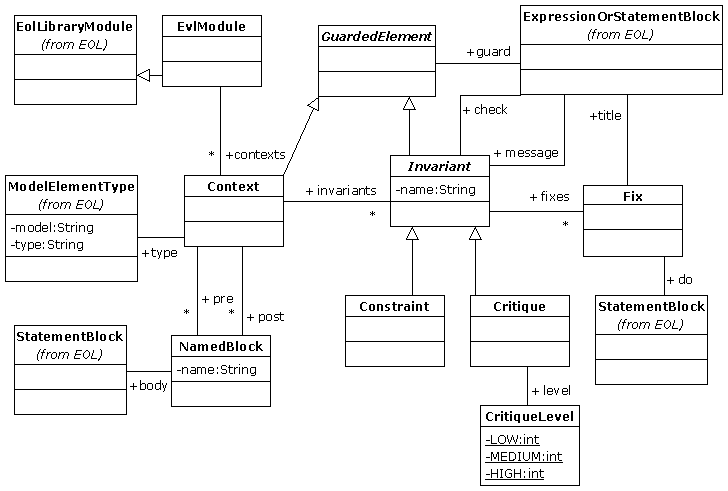
\includegraphics{images/EvlAbstractSyntax.png}
	\caption{Abstract Syntax of EVL}
	\label{fig:EvlAbstractSyntax}
\end{sidewaysfigure}
%\end{landscape}

\paragraph{Context} A context specifies the kind of instances on which the contained invariants will be evaluated. Each context can optionally define a guard which limits its applicability to a narrower subset of instances of its specified type. Thus, if the guard fails for a specific instance of the type, none of its contained invariants are evaluated.

\paragraph{Invariant} As with OCL, each EVL invariant defines a \emph{name} and a body (\emph{check}). However, it can optionally also define a \emph{guard} (defined in its abstract \emph{GuardedElement} supertype) which further limits its applicability to a subset of the instances of the type defined by the embracing \emph{context}. To achieve the requirement for detailed user feedback (Section \ref{sec:Issue1}), each invariant can optionally define a \emph{message} as an \emph{ExpressionOrStatementBlock} that should return a String providing a description of the reason(s) for which the constraint has failed on a particular element. To support semi-automatically fixing of elements on which invariants have failed (Section \ref{sec:Issue5}), an invariant can optionally define a number of \emph{fixes}. Finally, as displayed in Figure \ref{fig:EvlAbstractSyntax}, \emph{Invariant} is an abstract class that is used as a super-class for the specific types \emph{Constraint} and \emph{Critique}. This is to address the issue of separation of errors and warnings/critiques (Section \ref{sec:Issue2}).

\paragraph{Guard} Guards are used to limit the applicability of invariants (Section \ref{sec:Issue4}). This can be achieved at two levels. At the \emph{Context} level it limits the applicability of all invariants of the context and at the \emph{Invariant} level it limits the applicability of a specific invariant.

\paragraph{Fix}
A fix defines a title using an \emph{ExpressionOrStatementBlock} instead of a static String to allow users to specify context-aware titles (e.g. \emph{Rename class customer to Customer} instead of a generic \emph{Convert first letter to upper-case}). Moreover, the \emph{do} part is a statement block where the fixing functionality can be defined using EOL. The developer is responsible for ensuring that the actions contained in the \emph{fix} actually repair the identified inconsistency.

\paragraph{Constraint}
\emph{Constraints} in EVL are used to capture critical errors that invalidate the model. As discussed above, \emph{Constraint} is a sub-class of \emph{Invariant} and therefore inherits all its features.

\paragraph{Critique}
Unlike \emph{Constraints}, \emph{Critiques} are used to capture non-critical situations that do not invalidate the model, but should nevertheless be addressed by the user to enhance the quality of the model. This separation addresses the issue raised in Section \ref{sec:Issue2}.

\paragraph{Pre and Post}
An EVL module can define a number of named \emph{pre} and a \emph{post} blocks that contain EOL statements which are executed before and after evaluating the invariants respectively. These should not be confused with the pre-/post-condition annotations available for EOL user-defined operations (Section~\ref{sec:prep-cond-user}).

\section{Concrete Syntax}

Listings \ref{lst:ContextConcreteSyntax}, \ref{lst:InvariantConcreteSyntax} and \ref{lst:FixConcreteSyntax} demonstrate the concrete sytnax of the \emph{context}, \emph{invariant} and \emph{fix} abstract syntax constructs discussed above.

\begin{lstlisting}[caption=Concrete Syntax of an EVL context, label=lst:ContextConcreteSyntax, language=EVL, escapechar=!]
(@lazy)?
context !\textit{<name>}! !\textbf{\{}!

	(guard (!\textbf{:}\textit{expression}!)|(!\textbf{\{}\textit{statementBlock}\textbf{\}}!))?
	
	(!\textit{invariant}!)*
	
!\textbf{\}}!
\end{lstlisting}

\begin{lstlisting}[caption=Concrete Syntax of an EVL invariant, label=lst:InvariantConcreteSyntax, language=EVL, escapechar=!]
(@lazy)?
(constraint|critique) !\textit{<name>}! !\textbf{\{}!
	
	(guard (!\textbf{:}\textit{expression}!)|(!\textbf{\{}\textit{statementBlock}\textbf{\}}!))?
	
	(check (!\textbf{:}\textit{expression}!)|(!\textbf{\{}\textit{statementBlock}\textbf{\}}!))?
	
	(message (!\textbf{:}\textit{expression}!)|(!\textbf{\{}\textit{statementBlock}\textbf{\}}!))?
	
	(!\textit{fix}!)*
	
!\textbf{\}}
\end{lstlisting}

\begin{lstlisting}[float=t, caption=Concrete Syntax of an EVL fix, label=lst:FixConcreteSyntax, language=EVL, escapechar=!]
fix !\textbf{\{}!
	(guard (!\textbf{:}\textit{expression}!)|(!\textbf{\{}\textit{statementBlock}\textbf{\}}!))?
	
	(title (!\textbf{:}\textit{expression}!)|(!\textbf{\{}\textit{statementBlock}\textbf{\}}!))
	
	do !\textbf{\{}!
		!\textit{statementBlock}!
	!\textbf{\}}!
	
!\textbf{\}}!
\end{lstlisting}

\emph{Pre} and \emph{post} blocks have a simple syntax that, as presented in Listing \ref{lst:EvlPrePostConcreteSyntax}, consists of the identifier (\emph{pre} or \emph{post}), an optional name and the set of statements to be executed enclosed in curly braces.

\begin{lstlisting}[float=t, caption=Concrete Syntax of Pre and Post blocks, label=lst:EvlPrePostConcreteSyntax, language=EVL]
(pre|post) <name> {
	statement+
}
\end{lstlisting}

%\subsection{Concepts reused from EOL}

%As EVL has been built atop EOL, it reuses the following constructs from the base-language:

%\paragraph{ExpressionOrStatementBlock} There are cases where users needs to calculate a value (e.g. in the \emph{message} of an \emph{invariant}, in the \emph{guard} of a \emph{context} etc). When the value can be calculated declaratively, this is preferred. However, for cases in which calculating the value requires complex computations, users can use an EOL statement block and use a \emph{ReturnStatement} to return the calculated value to the caller.

%\paragraph{StatementBlock} A statement block is a sequence of EOL statements that can optionally include one or more \emph{ReturnStatements} to return a calculated value to its caller.

\section{Execution Semantics}
\label{sec:Design.EVL.ExecutionSemantics}

Having discussed the abstract and concrete syntaxes of EVL, this section provides an informal discussion of the execution semantics of the language. The execution of an EVL module is separated into four phases:

%The additional concepts EVL provides also affect its execution semantics. Currently, an EVL module can only be executed in batch-mode (all invariants against all instances). In the future we plan to investigate how the additional structures that EVL provides affect approaches to incremental consistency checking such as those presented in \cite{Cabot06,Egyed06}. In this section we outline the execution semantics of the language in batch-mode.

\paragraph{Phase 1} Before any invariant is evaluated, the \emph{pre} sections of the module are executed in the order in which they have been specified.

\paragraph {Phase 2} For each non-lazy \emph{context} with at least one non-lazy invariant, the instances of the meta-class it defines are collected. For each instance, the \emph{guard} of the \emph{context} is evaluated. If the \emph{guard} is satisfied, then for each non-lazy invariant contained in the context the invariant's \emph{guard} is also evaluated. If the \emph{guard} of the invariant is satisfied, the \emph{body} of the invariant is evaluated. In case the \emph{body} evaluates to \emph{false}, the \emph{message} part of the rule is evaluated and the produced message is added along with the instance, the invariant and the available \emph{fixes} to the \emph{ValidationTrace}.

The execution order of an EVL module follows a top-down depth-first scheme that respects the order in which the \emph{contexts} and \emph{invariants} appear in the module. However, the execution order can change in case one of the \emph{satisfies}, \emph{satisfiesOne}, \emph{satisfiesAll} built-in operations, discussed in detail in the sequel, are called.

\paragraph{Phase 3} In this phase, the validation trace is examined for unsatisfied constraints and the user is presented with the message each one has produced. The user can then select one or more of the available \emph{fixes} to be executed. Execution of \emph{fixes} is performed in a transactional manner using the respective facilities provided by the model connectivity framework, as discussed in Section \ref{sec:EMC.ModelTransactionSupport}. This is to prevent runtime errors raised during the execution of a \emph{fix} from compromising the validated model by leaving it in an inconsistent state.

\paragraph{Phase 4} When the user has performed all the necessary \emph{fixes} or chooses to end Phase 3 explicitly, the \emph{post} section of the module is executed. There, the user can perform tasks such as serializing the validation trace or producing a summary of the validation process results.

\subsection{Capturing Dependencies Between Invariants}

As discussed in Section \ref{sec:Issue3}, it is often the case that invariants conceptually depend on each other. To allow users capture such dependencies, EVL provides the \emph{satisfies(invariant : String) : Boolean}, \emph{satisfiesAll(invariants : Sequence(String)) : Boolean} and \emph{satisfiesOne(invariants : Sequence(String)) : Boolean} built-in operations. Using these operations, an invariant can specify in its \emph{guard} other invariants which need to be satisfied for it to be meaningful to evaluate.

When one of these operations is invoked, if the required \emph{invariants} (either lazy or non-lazy) have been evaluated for the instances on which the operation is invoked, the engine will return their cached results; otherwise it will evaluate them and return their results.

\section{Intra-Model Consistency Checking Example}
\label{sec:EvlIntraModelExample}
This section presents a case study comparing EVL and OCL in the context of a common scenario. The purpose of the case study is to present readers with the concrete syntax of the language and demonstrate the benefits delivered by the additional constructs it facilitates.

\subsection{Scenario: The Singleton Pattern}

The \emph{singleton} pattern is a widely used object oriented pattern. A \emph{singleton} is a class for which \emph{exactly one instance is allowed} \cite{Larman}. In UML, a singleton is typically represented as a class which is stereotyped with a \verb|<<singleton>>| stereotype and which also defines a static operation named \emph{getInstance()} that returns the unique instance. 

To ensure that all singletons have been modelled correctly in a UML model one needs to evaluate the following invariants on all classes that are stereotyped with the \verb|<<singleton>>| stereotype:

\begin{itemize}
	\item DefinesGetInstance : Each stereotyped class must define a getInstance() method
	\item GetInstanceIsStatic : The getInstance() method must be static
	\item GetInstanceReturnsSame : The return type of the getInstance() method must be the class itself 
\end{itemize}

Obviously, invariants \emph{GetInstanceIsStatic} and \emph{GetInstanceReturnsSame} depend on \emph{DefinesGetInstance} because if the singleton does not define a \emph{getInstance()} operation, checking for the operation's scope and return type is meaningless. Moreover, in case an invariant fails, there are corrective actions (fixes) that users may want to perform semi-automatically: e.g. for \emph{DefinesGetInstance}, such an action would be to add the missing \emph{getInstance()} operation, for \emph{GetInstanceIsStatic} to change it to static and for \emph{GetInstanceRetunrsSame} to set the return type to the class itself. In the following sections OCL and EVL are used to express the three constraints and then the two solutions are compared.

\subsection{Using OCL to Express the Invariants}

Listing \ref{lst:CaseStudyOcl} shows the aforementioned invariants implemented in OCL.

\begin{lstlisting}[basicstyle=\ttfamily\footnotesize, flexiblecolumns=true, numbers=none, nolol=true, caption=OCL Module for Validating Singletons, label=lst:CaseStudyOcl, numbers=left, language=OCL2, tabsize=2]
package Foundation::Core
    
		context Class 

		def isSingleton :
			let isSingleton : Boolean =
			self.stereotype->exists(s|s.name = 'singleton')
        
		def getInstanceOperation  : 
			let getInstanceOperation : Operation =
			self.feature->select(f|f.oclIsTypeOf(Operation) 
			and f.name = 'getInstance')->first().oclAsType(Operation)

		inv DefinesGetInstanceOperation : 
			if isSingleton 
				then getInstanceOperation.isDefined
				else true
			endif
    	
		inv GetInstanceOperationIsStatic :
			if isSingleton then
				if getInstanceOperation.isDefined 
					then getInstanceOperation.ownerScope = #classifier 
					else false
				endif
			else 
				true
			endif
    	
		inv GetOperationReturnsSame :
			if isSingleton then
				if getInstanceOperation.isDefined then
					if getInstanceOperation.returnParameter.isDefined
						then getInstanceOperation.returnParameter.type = self 
						else false
					endif
				else
					false
				endif
			else 
				true
			endif
    	
    context Operation
        
		def returnParameter :
			let returnParameter : Parameter =
			self.parameter->select(p|p.kind = #return)->first()

endpackage

\end{lstlisting}

By examining the OCL solution it can be observed that all invariants first check that the class is a singleton (lines 15, 21 and 31) by using the \emph{isSingleton} derived property defined in line 5. If the isSingleton returns \emph{false}, the invariants return \emph{true} since returning false would cause them to fail for all non-singleton classes. This reveals an additional shortcoming of OCL: if a constraint returns \emph{true} it may mean two different things: either that the instance satisfies the constraint or that the constraint is not applicable to the instance at all. In our view, this overloading reduces understandability.

By further studying the solution of Listing \ref{lst:CaseStudyOcl} it can be noticed that dependency between constraints is captured artificially using nested \emph{if} expressions. For instance, both \emph{GetInstanceIsStatic} and \emph{GetInstanceRetunrsSame} contain an \emph{if} expression in lines 22 and 32 respectively, requiring that they recalculate the value of the \emph{getInstanceOperation} defined in line 9, where they actually recalculate the result of the \emph{DefinesGetInstanceOperation} invariant. As discussed in Section \ref{sec:Issue3}, this happens because OCL lacks constructs for capturing dependencies in a structured manner.

\subsection{Using EVL to Express the Invariants}

Listing \ref{lst:CaseStudy} provides a solution for this problem expressed in EVL.

\begin{lstlisting}[basicstyle=\ttfamily\footnotesize, flexiblecolumns=true, numbers=none, nolol=true, caption=EVL Module for Validating Singletons, label=lst:CaseStudy, numbers=left, language=EVL, tabsize=2]
context Singleton typeOf Class {
	
	guard : self.stereotype->exists(s|s.name = 'singleton')
	
	constraint DefinesGetInstance {
		check : self.getGetInstanceOperation()->isDefined()
		message : 'Singleton ' + self.name + 
			' must define a getInstance() operation'
		fix {
			title : 'Add a getInstance() operation to ' + self.name
			do {
				-- Create the getInstance operation
				var op : new Operation;
				op.name := 'getInstance';
				op.owner := self;
				op.ownerScope := ScopeKind#sk_classifier;
				
				-- Create the return parameter
				var returnParameter : new Parameter;
				returnParameter.type := self;
				op.parameter := Sequence{returnParameter};
				returnParameter.kind := ParameterDirectionKind#pdk_return;
			}
		}
	}
	
	constraint GetInstanceIsStatic {
		guard : self.satisfies('DefinesGetInstance')
		check : self.getGetInstanceOperation().ownerScope = 
		        ScopeKind#sk_classifier
		message : ' The getInstance() operation of singleton ' 
		          + self.name + ' must be static'
	
		fix {
			title : 'Change to static'
			do {
				self.getGetInstanceOperation.ownerScope 
				  := ScopeKind#sk_classifier;
			}
		}
	}
	
	constraint GetInstanceReturnsSame {
	
		guard : self.satisfies('DefinesGetInstance')
		check {
			var returnParameter : Parameter;
			returnParameter := self.getReturnParameter();
			return (returnParameter->isDefined() 
			        and returnParameter.type = self);
		}
		message : ' The getInstance() operation of singleton ' 
		          + self.name + ' must return ' + self.name
			
		fix {
			title : 'Change return type to ' + self.name
			do {
				var returnParameter : Parameter;
				returnParameter := self.getReturnParameter();
				
				-- If the operation does not have a return parameter
				-- create one
				if (not returnParameter.isDefined()){
					returnParameter := Parameter.newInstance();
					returnParameter.kind := ParameterDirectionKind#pdk_return;
					returnParameter.behavioralFeature := 
						self.getInstanceOperation();
				}
				-- Set the correct return type
				returnParameter.type := self;
			}
		}
	}
}

operation Class getGetInstanceOperation() : Operation {
	return self.feature->
		select(o:Operation|o.name = 'getInstance').first();
}

operation Operation getReturnParameter() : Parameter {
	return self.parameter->
		select(p:Parameter|p.kind = 
			ParameterDirectionKind#pdk_return).first();
}
\end{lstlisting}

The \emph{Singleton} context defines that the invariants it contains will be evaluated on instances of the UML \emph{Class} type. Moreover, its guard defines that they will be evaluated only on classes that are stereotyped with the \emph{singleton} stereotype. Therefore, unlike the OCL solution of Listing \ref{lst:CaseStudyOcl}, invariants contained in this context do not need to check individually that the instances on which they are evaluated are singletons.

Constraint \emph{DefinesGetInstance} defines no guard which means that it will be evaluated for all the instances of the context. In its \emph{check} part, the constraint examines if the class defines an operation named \emph{getInstance()} by invoking the \emph{getGetInstanceOperation()} operation. If this fails, it proposes a fix that adds the missing operation to the class.

Constraint \emph{GetInstanceIsStatic} defines a guard which states that for the constraint to be evaluated on an instance, the instance must first satisfy the \emph{DefinesGetInstance} constraint. If it doesn't, it is not evaluated at all. In its \emph{check} part it examines that the \emph{getInstance()} operation is static. Note that here the constraint needs not check that the \emph{getInstance()} operation is defined again since this is assumed by the \emph{DefinesGetInstance} constraint on which it depends. If the constraint fails for an instance, the fix part can be invoked to change the scope of the \emph{getInstance()} operation to static.

Constraint \emph{GetInstanceReturnsSame} checks that the return type of the \emph{getInstance()} operation is the singleton itself. Similarly to the \emph{GetInstanceIsStatic} constraint, it defines that to be evaluated the \emph{DefinesGetInstance} constraint must be satisfied. If it fails for a particular instance, the fix part can be invoked. In the fix part, if the operation defines a return parameter of incorrect type, its type is changed and if it does not define a return parameter at all, the parameter is created and added to the parameters of the operation.

By observing the two solutions the OCL solution resembles the concept of defensive programming, where conditions are embedded in supplier code, while the EVL one is closer to the design by contract \cite{Meyer97} approach where conditions are explicitly checked in guards.

This case study has demonstrated that the additional constructs provided by EVL can reduce repetition significantly and thus enable specification of more concise constraints. Moreover, in case a constraint is not satisfied for a particular instance, the user is provided with a meaningful context-aware message and with automated facilities (fixes) for repairing the inconsistency.

\section{Inter-Model Consistency Checking Example}
\label{sec:EvlInterModelExample}

\begin{figure}[b]
	\centering
		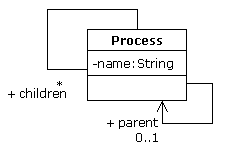
\includegraphics{images/Process.png}
	\caption{The ProcessLang Metamodel}
	\label{fig:Process}
\end{figure}

In the previous example, EVL was used to check the internal consistency of a single UML model. By contrast, this example demonstrates using EVL to detect and repair occurrences of incompleteness and contradiction between two different models. In this example the simplified \emph{ProcessLang} metamodel, which captures information about hierarchical processes, is used. To add performance information in a separate aspect \emph{ProcessPerformanceLang} metamodel is also defined. The metamodels are displayed in Figures \ref{fig:Process} and \ref{fig:ProcessPerformance} respectively.

\begin{figure}[h]
	\centering
		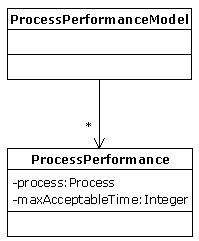
\includegraphics[width=0.2\textwidth]{images/ProcessPerformance.png}
	\caption{The ProcessPerformanceLang Metamodel}
	\label{fig:ProcessPerformance}
\end{figure}

There are two constraints that need to be defined and evaluated in this example: that each \emph{Process} in a process model (\emph{PM}) has a corresponding \emph{ProcessPerformance} in the process performance model (\emph{PPM}), and that the \emph{maxAcceptableTime} of a process does not exceed the sum of the \emph{maxAcceptableTimes} of its children. This is achieved with the \emph{PerformanceIsDefined} and the \emph{PerformanceIsValid} EVL constraints displayed in Listing \ref{lst:InterModelCaseStudy}.


\begin{lstlisting}[caption=Exemplar EVL module containing a cross-model constraint, label=lst:InterModelCaseStudy, language=EVL]
context PM!Process {	
	constraint PerformanceIsDefined { /*@\label{CaseStudy:PerformanceIsDefined}@*/
		
		check { /*@\label{CaseStudy:PerformanceIsDefined:Check}@*/
			var processPerformances = 
				PPM!ProcessPerformance.
				allInstances.select(pt|pt.process = self);
			
			return processPerformances.size() = 1;
		}
		
		message { /*@\label{CaseStudy:PerformanceIsDefined:Message}@*/
			var prefix : String;
			if (processPerformances.size() = 1) {
				prefix = "More than one performance info"; 
			}
			else {
				prefix = "No performance info";
			}
			return prefix + " found for process " 
				+ self.name;
		}
		
		fix { /*@\label{CaseStudy:PerformanceIsDefined:Fix}@*/
			title : "Set the performance of " + self.name
			
			do {
				for (p in processPerformances.clone()) {
					delete p;
				}
				var maxAcceptableTime : Integer;
				maxAcceptableTime = UserInput. /*@\label{CaseStudy:PerformanceIsDefined:Fix:Prompt}@*/
					promptInteger("maxAcceptableTime", 0); 
				var p : 
					new PPM!ProcessPerformance;
				p.maxAcceptableTime = maxAcceptableTime;
				p.process = self;
			}
		}
	}
	
	constraint PerformanceIsValid { /*@\label{CaseStudy:PerformanceIsValid}@*/
		
		guard : self.satisfies("PerformanceIsDefined") /*@\label{CaseStudy:PerformanceIsValid:Guard}@*/
			and self.children.forAll
				(c|c.satisfies("PerformanceIsDefined"))
		
		check { /*@\label{CaseStudy:PerformanceIsValid:Check}@*/
			var sum : Integer;
			sum = self.children. /*@\label{CaseStudy:PerformanceIsValid:Sum}@*/
				collect(c|c.getMaxAcceptableTime()) 
				.sum().asInteger(); 
			return self.getMaxAcceptableTime() >= sum;
		}
		
		message : "Process " + self.name + /*@\label{CaseStudy:PerformanceIsValid:Message}@*/
			" has a smaller maxAcceptableTime " 
			+ "than the sum of its children"
		
		fix { /*@\label{CaseStudy:PerformanceIsValid:Fix}@*/
			title : "Increase maxAcceptableTime to " + sum
			do {
				self.setMaxAcceptableTime(sum);
			}
		}
		
	}
	
}

operation PM!Process getMaxAcceptableTime() /*@\label{CaseStudy:getMaxAcceptableTime}@*/
	: Integer { 
	return PPM!ProcessPerformance.
		allInstances.selectOne(pt|pt.process=self)
			.maxAcceptableTime;
}

operation PM!Process setMaxAcceptableTime /*@\label{CaseStudy:setMaxAcceptableTime}@*/
	(time : Integer) { 
	PPM!ProcessPerformance.allInstances.
		selectOne(pt|pt.process=self).maxAcceptableTime =
		time;
}
\end{lstlisting}

In line \ref{CaseStudy:PerformanceIsDefined:Check}, the check part of the \emph{PerformanceIsDefined} constraint calculates the instances of \emph{ProcessPerformance} in the \emph{ProcessPerformanceModel} that have their \emph{process} reference set to the currently examined \emph{Process} (accessible via the \emph{self} built-in variable) and stores it in the \emph{processPerformances} variable. If exactly one \emph{ProcessPerformance} is defined for the \emph{Process}, the constraint is satisfied. Otherwise, the \emph{message} part of the constraint, in line \ref{CaseStudy:PerformanceIsDefined:Message}, is evaluated and an appropriate error message is displayed to the user. 

Note that the \emph{processPerformances} variable defined in the \emph{check} part is also used from within the \emph{message} part of the constraint. As discussed in \cite{EVL}, EVL provides this feature to reduce the need for duplicate calculations as our experience has shown that the message for a failed constraint often needs to utilize side-information collected in the \emph{check} part.

To repair the inconsistency, the user can invoke the \emph{fix} defined in line \ref{CaseStudy:PerformanceIsDefined:Fix} that will delete any existing \emph{ProcessPerformance} instances and create a new one with a user-defined \emph{maxAcceptableTime} obtained using the \emph{UserInput.promptInteger()} statement of line \ref{CaseStudy:PerformanceIsDefined:Fix:Prompt}.

Unlike the \emph{PerformanceIsDefined} constraint, the \emph{PerformanceIsValid} constraint, line \ref{CaseStudy:PerformanceIsValid}, defines a \emph{guard} part (line \ref{CaseStudy:PerformanceIsValid:Guard}). As discussed in \cite{EVL}, the guard part of a constraint is used to further limit the applicability of the constraint beyond the simple type check performed in the containing \emph{context}. In this rule, the validity of the \emph{maxAcceptableTime} of a \emph{Process} needs to be checked only if one has been defined in the \emph{ProcessPerformanceModel}. Therefore, the guard part of the constraint specifies that this constraint is only applicable to \emph{Processes} where, both they and they children, satisfy the \emph{PerformanceIsDefined} constraint.

The check part of the constraint retrieves the \emph{maxAcceptableTime} of the process and that of its children and compares them. As the \emph{Process} itself does not define performance information, retrieval of the value of the \emph{maxAcceptableTime} of the respective \emph{ProcessPerformance} object is implemented using the user-defined \emph{getMaxAcceptableTime()} operation that is defined in line \ref{CaseStudy:getMaxAcceptableTime}. In case the constraint is not satisfied, the user can invoke the \emph{fix} defined in line \ref{CaseStudy:PerformanceIsValid:Fix} to repair the inconsistency by setting the \emph{maxAcceptableTime} of the process to the \emph{sum} calculated in line \ref{CaseStudy:PerformanceIsValid:Sum}. As discussed earlier, the fix parts of EVL invariants do not in any way guarantee that they do fix the problem they target or that in their effort to fix one problem they do not create another problem; this is left to the user. For instance, in this particular example, changing the \emph{maxAcceptableTime} of a process through a \emph{fix} block may render its parent process invalid.


To demonstrate the evaluation of these constraints two exemplar models that conform to the \emph{ProcessLang} and \emph{ProcessPerformanceLang} metamodels are used. A visual representation of the models is displayed in Figure \ref{fig:ModeLink}.

\begin{figure}[h]
    \centering
    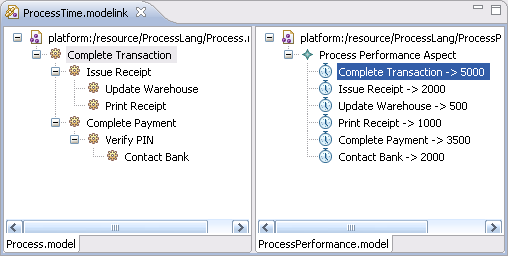
\includegraphics{images/ModeLink.png}
    \caption{Exemplar Process and ProcessPerformance models}
    \label{fig:ModeLink}
\end{figure}


Evaluating the constraints in the context of those two models reveals two problems which are reported to the user via the view displayed in Figure \ref{fig:Validation}. Indeed by examining the two models of Figure \ref{fig:ModeLink}, it becomes apparent that there is no \emph{ProcessPerformance} linked to the \emph{Verify PIN} process and also that the \emph{maxAcceptableTime} of \emph{Complete Transaction} (5000) is less than the sum of the \emph{maxAcceptableTimes} of its children (2000 + 3500).

\begin{figure}[h]
    \centering
    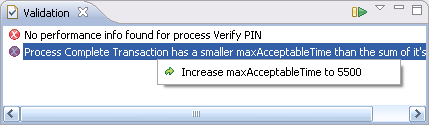
\includegraphics{images/Validation.png}
    \caption{Screenshot of the validation view reporting the identified inconsistencies}
    \label{fig:Validation}
\end{figure}

\section{Summary}

This section has provided a detailed discussion on the EVL model-validation language which conceptually (as opposed to technically) extends OCL. EVL provides a number of features such as support for detailed user feedback, constraint dependency management, semi-automatic transactional inconsistency resolution and (as it is based on EOL) access to multiple models of diverse metamodels and technologies.

%%% Local Variables:
%%% mode: latex
%%% TeX-master: "EpsilonBook"
%%% End:


\chapter{The Epsilon Transformation Language (ETL)}
\label{sec:ETL}

The aim of ETL \cite{ETL} is to contribute model-to-model transformation capabilities to Epsilon. More specifically, ETL can be used to transform an arbitrary number of input models into an arbitrary number of output models of different modelling languages and technologies at a high level of abstraction. 

\section{Style}

Three styles are generally recognized in model transformation languages: declarative, imperative and hybrid, each one demonstrating particular advantages and shortcomings. Declarative transformation languages are generally limited to scenarios where the source and target metamodels are similar to each other in terms of structure and thus, the transformation is a matter of a simple mapping. However they fail to address cases where significant processing and complex mappings are involved. On the other hand, purely imperative transformation languages are capable of addressing a wider range of transformation scenarios. Nevertheless, they operate at a low level of abstraction which means that users need to manually address issues such as tracing and resolving target elements from their source counterparts and orchestrating the transformation execution. To address those shortcomings, hybrid languages (such as ATL \cite{ATL} and QVT \cite{QVT}) provide both a declarative rule-based execution scheme as well as imperative features for handling complex transformation scenarios. 

Under this rationale, ETL has been designed as a hybrid language that implements a task-specific rule definition and execution scheme but also inherits the imperative features of EOL to handle complex transformations where this is deemed necessary.

\section{Source and Target Models}

The majority of model-to-model transformation languages assume that only two models participate in each transformation: the source model and the target model. Nevertheless, it is often essential to be able to access/update additional models during a transformation (such as trace or configuration models). Building on the facilities provided by EMC and EOL, ETL enables specification of transformations that can transform an arbitrary number of source models into an arbitrary number of target models.

Another common assumption is that the contents of the target models are insignificant and thus a transformation can safely overwrite its contents. As discussed in the sequel, ETL - like all Epsilon languages - enables the user to specify, for each involved model, whether its contents need to be preserved or not.

\section{Abstract Syntax}

As illustrated in Figure \ref{fig:EtlAbstractSyntax}, ETL transformations are organized in modules (\emph{EtlModule}). A module can contain a number of transformation rules (\emph{TransformationRule}). Each rule has a unique name (in the context of the module) and also specifies one \emph{source} and many \emph{target} parameters. A transformation rule can also \emph{extend} a number of other transformation rules and be declared as \emph{abstract}, \emph{primary} and/or \emph{lazy}\footnote{The concept of lazy rules was first introduced in ATL}. To limit its applicability to a subset of elements that conform to the type of the \emph{source} parameter, a rule can optionally define a guard which is either an EOL expression or a block of EOL statements. Finally, each rule defines a block of EOL statements (\emph{body}) where the logic for populating the property values of the target model elements is specified.

Besides transformation rules, an ETL module can also optionally contain a number of \emph{pre} and \emph{post} named blocks of EOL statements which, as discussed later, are executed before and after the transformation rules respectively. These should not be confused with the pre-/post-condition annotations available for EOL user-defined operations (Section~\ref{sec:prep-cond-user}).

\begin{landscape}
\begin{figure}
	\centering
		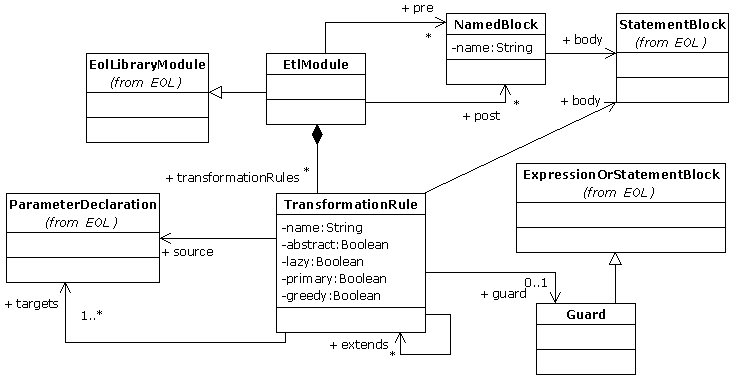
\includegraphics{images/EtlAbstractSyntax.png}
	\caption{ETL Abstract Syntax}
	\label{fig:EtlAbstractSyntax}
\end{figure}
\end{landscape}

\section{Concrete Syntax}

The concrete syntax of a transformation rule is displayed in Listing \ref{lst:TransformationRuleConcreteSyntax}. The optional \emph{abstract}, \emph{lazy} and \emph{primary} attributes of the rule are specified using respective annotations. The name of the rule follows the \emph{rule} keyword and the \emph{source} and \emph{target} parameters are defined after the \emph{transform} and \emph{to} keywords. Also, the rule can define an optional comma-separated list of rules it extends after the \emph{extends} keyword. Inside the curly braces (\{\}), the rule can optionally specify its \emph{guard} either as an EOL expression following a colon (:) (for simple guards) or as a block of statements in curly braces (for more complex guards). Finally, the \emph{body} of the rule is specified as a sequence of EOL statements.

\begin{lstlisting}[caption=Concrete Syntax of a TransformationRule, label=lst:TransformationRuleConcreteSyntax, language=ETL]
(@abstract)?
(@lazy)?
(@primary)?
rule <name> 
	transform <sourceParameterName>:<sourceParameterType>
	to (<rightParameterName>:<rightParameterType>
	(, <rightParameterName>:<rightParameterType>)*
	(extends (<ruleName>,)*<ruleName>)? {
	
	(guard (:expression)|({statement+}))?
	
	statement+
}
\end{lstlisting}

\emph{Pre} and \emph{post} blocks have a simple syntax that, as presented in Listing \ref{lst:EtlPrePostConcreteSyntax}, consists of the identifier (\emph{pre} or \emph{post}), an optional name and the set of statements to be executed enclosed in curly braces.

\begin{lstlisting}[caption=Concrete Syntax of Pre and Post blocks, label=lst:EtlPrePostConcreteSyntax, language=ETL]
(pre|post) <name> {
	statement+
}
\end{lstlisting}

\section{Execution Semantics}
\label{sec:ETL.ExecutionSemantics}

\subsection{Rule and Block Overriding}
Similarly to ECL, an ETL module can import a number of other ETL modules. In this case, the importing ETL module inherits all the rules and pre/post blocks specified in the modules it imports (recursively). If the module specifies a rule or a pre/post block with the same name, the local rule/block overrides the imported one respectively.

\subsection{Rule Execution Scheduling}

When an ETL module is executed, the \emph{pre} blocks of the module are executed first in the order in which they have been specified. 

Following that, each \emph{non-abstract} and \emph{non-lazy} rule is executed for all the elements on which it is applicable. To be applicable on a particular element, the element must have a kind-of relationship with the type defined in the rule's \emph{sourceParameter} and must also satisfy the \emph{guard} of the rule (and all the rules it extends). When a rule is executed on an applicable element, the target elements are initially created by instantiating the \emph{targetParameters} of the rules, and then their contents are populated using the EOL statements of the \emph{body} of the rule.

Finally, when all rules have been executed, the \emph{post} blocks of the module are executed in the order in which they have been declared.

\subsection{Source Elements Resolution}

Resolving target elements that have (or can be) transformed from source elements by other rules is a frequent task in the body of a transformation rule. To automate this task and reduce coupling between rules, ETL contributes the \emph{equivalents()} and \emph{equivalent()} built-in operations that automatically resolve source elements to their transformed counterparts in the target models. 

When the \emph{equivalents()} operation is applied on a single source element (as opposed to a collection of them), it inspects the established transformation trace (displayed in Figure \ref{fig:EtlRuntime}) and invokes the applicable rules (if necessary) to calculate the counterparts of the element in the target model. When applied to a collection it returns a \emph{Bag} containing \emph{Bags} that in turn contain the counterparts of the source elements contained in the collection. The \emph{equivalents()} operation can be also invoked with an arbitrary number of rule names as parameters to invoke and return only the equivalents created by specific rules. Unlike the main execution scheduling scheme discussed above, the \emph{equivalents()} operation invokes both \emph{lazy} and \emph{non-lazy} rules. It is worth noting that \emph{lazy} rules are computationally expensive and should be used with caution as they can significantly degrade the performance of the overall transformation.

With regard to the ordering of the results of the \emph{equivalents()} operations, the returned elements appear in the respective order of the rules that have created them. An exception to this occurs when one of the rules is declared as \emph{primary}, in which case its results precede the results of all other rules.

\begin{landscape}
\begin{figure}
	\centering
		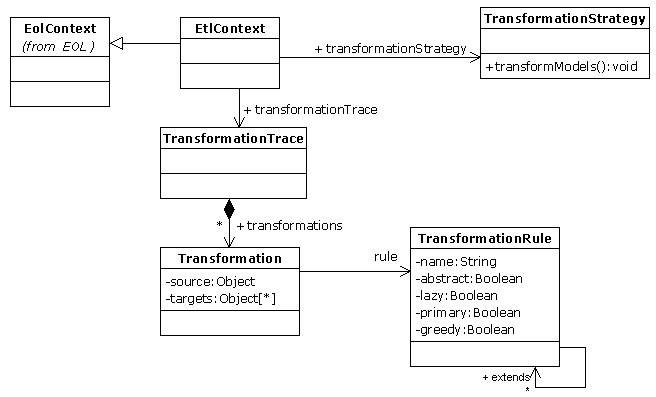
\includegraphics{images/EtlRuntime.png}
	\caption{ETL Runtime}
	\label{fig:EtlRuntime}
\end{figure}
\end{landscape}


ETL also provides the convenience \emph{equivalent()} operation which, when applied to a single element, returns only the first element of the respective result that would have been returned by the \emph{equivalents()} operation discussed above. Also, when applied to a collection the \emph{equivalent()} operation returns a flattened collection (as opposed to the result of \emph{equivalents()} which is a \emph{Bag} of \emph{Bags} in this case). As with the \emph{equivalents()} operation, the \emph{equivalent()} operation can also be invoked with or without parameters.

The semantics of the \emph{equivalent()} operation are further illustrated through a simple example. In this example, we need to transform a model that conforms to the Tree metamodel displayed in Figure \ref{fig:Tree} into a model that conforms to the Graph metamodel of Figure \ref{fig:Graph}. More specifically, we need to transform each \emph{Tree} element to a \emph{Node}, and an \emph{Edge} that connects it with the \emph{Node} that is equivalent to the tree's \emph{parent}. This is achieved using the rule of Listing \ref{lst:SimpleETLTransformationRule}. 

\begin{lstlisting}[float=h, caption=Exemplar ETL Rule demonstrating the \emph{equivalent()} operation, label=lst:SimpleETLTransformationRule, language=ETL, escapechar=\#]
rule Tree2Node#\label{lst:etl-simple-def-start}#
	transform t : Tree!Tree
	to n : Graph!Node {#\label{lst:etl-simple-def-end}#
	
	n.label = t.label;#\label{lst:etl-simple-label}#
	
	if (t.parent.isDefined()) {#\label{lst:etl-simple-sourceisdef}#
		var edge = new Graph!Edge;#\label{lst:etl-simple-newedge}#
		edge.source = n;#\label{lst:etl-simple-source}#
		edge.target = t.parent.equivalent();#\label{lst:etl-simple-equiv}#
	}
}
\end{lstlisting}


In lines \ref{lst:etl-simple-def-start}--\ref{lst:etl-simple-def-end}, the \emph{Tree2Node} rule specifies that it can transform elements of the \emph{Tree} type in the \emph{Tree} model into elements of the \emph{Node} type in the \emph{Graph} model. In line~\ref{lst:etl-simple-label} it specifies that the name of the created Node should be the same as the name of the source Tree. If the parent of the source \emph{Tree} is defined (line~\ref{lst:etl-simple-sourceisdef}), the rule creates a new \emph{Edge} (line~\ref{lst:etl-simple-newedge}) and sets its \emph{source} property to the created \emph{Node} (line~\ref{lst:etl-simple-source}) and its \emph{target} property to the \emph{equivalent} \emph{Node} of the source \emph{Tree}'s \emph{parent} (line~\ref{lst:etl-simple-equiv}).

\begin{figure}
	\centering
		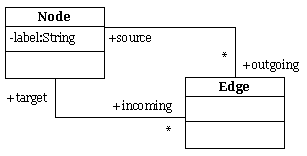
\includegraphics{images/Graph.png}
	\caption{A Simple Graph Metamodel}
	\label{fig:Graph}
\end{figure}


\subsection{Overriding the semantics of the EOL SpecialAssignmentOperator}
\label{sec:Design.ETL.SpecialAssignmentOperator}

As discussed above, resolving the equivalent(s) or source model elements in the target model is a recurring task in model transformation. Furthermore, in most cases resolving the equivalent of a model element is immediately followed by assigning/adding the obtained target model elements to the value(s) of a property of another target model element. For example, in line 10 of Listing \ref{lst:SimpleETLTransformationRule} the \emph{equivalent} obtained is immediately assigned to the \emph{target} property of the generated \emph{Edge}. To make transformation specifications more readable, ETL overrides the semantics of the \emph{SpecialAssignmentStatement} (\emph{::=} in terms of concrete syntax), described in Section \ref{sec:Design.EOL.SpecialAssignmentStatement} to set its left-hand side, not to the element its right-hand side evaluates to, but to its \emph{equivalent} as calculated using the \emph{equivalent()} operation discussed above. Using this feature, line 10 of the \emph{Tree2Node} rule can be rewritten as shown in Listing \ref{lst:SpecialAssignmentETLTransformationRule}

\begin{lstlisting}[caption=Rewritten Line 10 of the \emph{Tree2Node} Rule Demonstrated in Listing \ref{lst:SimpleETLTransformationRule}, label=lst:SpecialAssignmentETLTransformationRule, language=ETL]
edge.target ::= t.parent;
\end{lstlisting}


\section{Interactive Transformations}
\label{sec:InteractiveModelTransformation}

Using the user interaction facilities of EOL discussed in Section \ref{sec:Design.EOL.UserInput}, an ETL transformation can become interactive by prompting the user for input during its execution. For example in Listing \ref{lst:InteractiveETLTransformationRule}, we modify the \emph{Tree2Node} rule originally presented in Listing \ref{lst:SimpleETLTransformationRule} by adding a \emph{guard} part that uses the user-input facilities of EOL (more specifically the \emph{UserInput.confirm(String,Boolean)} operation) to enable the user select manually at runtime which of the Tree elements need to be transformed to respective Node elements in the target model and which not. 

\begin{lstlisting}[caption=Exemplar Interactive ETL Transformation, label=lst:InteractiveETLTransformationRule, language=ETL]
rule Tree2Node
	transform t : Tree!Tree
	to n : Graph!Node {
	
	guard : UserInput.confirm
		("Transform tree " + t.label + "?", true)
	
	n.label = t.label;
	var target : Graph!Node ::= t.parent;
	if (target.isDefined()) {
		var edge = new Graph!Edge;
		edge.source = n;
		edge.target = target;
	}
}
\end{lstlisting}

\section{Summary}

This section has provided a detailed discussion on the Epsilon Transformation Language (ETL). ETL is capable of transforming an arbitrary number of source models into an arbitrary number of target models. ETL adopts a hybrid style and features declarative rule specification using advanced concepts such as \emph{guards}, \emph{abstract}, \emph{lazy} and \emph{primary} rules, and automatic resolution of target elements from their source counterparts. Also, as ETL is based on EOL reuses its imperative features to enable users to specify particularly complex, and even interactive, transformations.

\chapter{The Epsilon Wizard Language (EWL)}
\label{sec:EWL}

There are two types of model-to-model transformations: mapping and update transformations \cite{Czarnecki2003}. Mapping transformations typically transform a source model into a set of target models expressed in (potentially) different modelling languages by creating zero or more model elements in the target models for each model element of the source model. By contrast, update transformations perform in-place modifications in the source model itself. They can be further classified into two subcategories: transformations in the small and in the large. Update transformations in the large apply to sets of model elements calculated using well-defined rules in a batch manner. An example of this category of transformations is a transformation that automatically adds accessor and mutator operations for all attributes in a UML model. On the other hand, update transformations in the small are applied in a user-driven manner on model elements that have been explicitly selected by the user. An example of this kind of transformations is a transformation that renames a \emph{user-specified} UML class and all its incoming associations consistently.

In Epsilon, mapping transformations can be specified using ETL as discussed in Section \ref{sec:ETL}, and update transformations in the large can be implemented either using the model modification features of EOL or using an ETL transformation in which the source and target models are the same model. By contrast, update transformations in the small cannot be effectively addressed by any of the languages presented so far.

The following section discusses the importance of update transformations in the small and motivates the definition of a task-specific language (Epsilon Wizard Language (EWL)) that provides tailored and effective support for defining and executing update transformations on models of diverse metamodels.

\section{Motivation}
\label{sec:EwlMotivation}

Constructing and refactoring models is undoubtedly a mentally intensive process. However, during modelling, recurring patterns of model update activities typically appear. As an example, when renaming a class in a UML class diagram, the user also needs to manually update the names of association ends that link to the renamed class. Thus, when renaming a class from \emph{Chapter} to \emph{Section}, all associations ends that point to the class and are named \emph{chapter} or \emph{chapters} should be also renamed to \emph{section} and \emph{sections} respectively. As another example, when a modeller needs to refactor a UML class into a singleton \cite{Larman}, they need to go through a number of well-defined, but trivial, steps such as attaching a stereotype ($<<singleton>>$), defining a static \emph{instance} attribute and adding a static \emph{getInstance()} method that returns the unique instance of the singleton.

It is generally accepted that performing repetitive tasks manually is both counter-productive and error-prone \cite{CG.InAction}. On the other hand, failing to complete such tasks correctly and precisely compromises the consistency, and thus the quality, of the models. In Model Driven Engineering, this is particularly important since models are increasingly used to automatically produce (parts of) working systems. 

\subsection{Automating the Construction and Refactoring Process}

Contemporary modelling tools provide built-in transformations (\textit{wizards}) for automating common repetitive tasks. However, according to the architecture of the designed system and the specific problem domain, additional repetitive tasks typically appear, which cannot be addressed by the pre-conceived built-in wizards of a modelling tool. To address the automation problem in its general case, users must be able to easily define update transformations (wizards) that are tailored to their specific needs.

To an extent, this can be achieved via the extensible architecture that state-of-the-art modelling tools often provide and which enables users to add functionality to the tool via scripts or application code using the implementation language of the tool. Nevertheless, as discussed in \cite{EOL}, the majority of modelling tools provide an API through which they expose an edited model, which requires significant effort to learn and use. Also, since each API is proprietary, such scripts and extensions are not portable to other tools. Finally, API scripting languages and third-generation languages such as Java and C++ are not particularly suitable for model navigation and modification \cite{EOL}.

Furthermore, existing languages for mapping transformations, such as QVT, ATL and ETL, cannot be used as-is for this purpose, because these languages have been designed to operate in a batch manner without human involvement in the process. By contrast, as discussed above, the task of constructing and refactoring models is inherently user-driven.

\section{Update Transformations in the Small}
\label{sec:ModelTransformationInTheSmall}

Update transformations are actions that automatically create, update or delete model elements based on a selection of existing elements in the model and information obtained otherwise (e.g. through user input), in a user-driven fashion. In this section such actions are referred to as \textit{wizards} instead of \textit{rules} to reduce confusion between them and rules of mapping transformation languages. In the following sections the desirable characteristics of wizards are elaborated informally. 

\subsection{Structure of Wizards}

In its simplest form, a wizard only needs to define the actions it will perform when it is applied to a selection of model elements. The structure of such a wizard that transforms a UML class into a \textit{singleton} is shown using pseudo-code in Listing \ref{lst:Basic}.\\

\begin{lstlisting}[caption=The simplest form of a wizard for refactoring a class into a singleton, label=lst:Basic, language=EWL]
do :
	attach the singleton stereotype
	create the instance attribute
	create the getInstance method
\end{lstlisting}

Since not all wizards apply to all types of elements in the model, each wizard needs to specify the types of elements to which it applies. For example, the wizard of Listing \ref{lst:Basic}, which automatically transforms a class into a singleton, applies only when the selected model element is a class. The simplest approach to ensuring that the wizard will only be applied on classes is to enclose its body in an \emph{if} condition as shown in Listing \ref{lst:WithoutGuard}.

\begin{lstlisting}[caption=The wizard of Listing \ref{lst:Basic} enhanced with an $if$ condition, label=lst:WithoutGuard, language=EWL]
do : 
	if (selected element is a class) {
		attach the singleton stereotype
		create the instance attribute
		create the getInstance method
	}
\end{lstlisting}

A more modular approach is to separate this condition from the body of the wizard. This is shown in Listing \ref{lst:WithGuard} where the condition of the wizard is specified as a separate \emph{guard} stating that the wizard applies only to elements of type Class. The latter is preferable since it enables filtering out wizards that are not applicable to the current selection of elements by evaluating only their \emph{guard} parts and rejecting those that return \emph{false}. Thus, at any time, the user can be provided with only the wizards that are applicable to the current selection of elements. Filtering out irrelevant wizards reduces confusion and enhances usability, particularly as the list of specified wizards grows.

\begin{lstlisting}[caption=The wizard of Listing \ref{lst:WithoutGuard} with an explicit $guard$ instead of the $if$ condition, label=lst:WithGuard, language=EWL]
guard : selected element is a class
do : 
	attach the singleton stereotype
	create the instance attribute
	create the getInstance method
\end{lstlisting}

To enhance usability, a wizard also needs to define a short human-readable description of its functionality. To achieve this, another field named \emph{title} has been added. There are two options for defining the title of a wizard: the first is to use a static string and the second to use a dynamic expression. The latter is preferable since it enables definition of context-aware titles.

\begin{lstlisting}[caption=The wizard of Listing \ref{lst:WithGuard} enhanced with a $title$ part, label=lst:FinalForm, language=EWL]
guard : selected element is a class
title : Convert class <class-name> into a singleton
do : 
	attach the singleton stereotype
	create the instance attribute
	create the getInstance method
\end{lstlisting}

\subsection{Capabilities of Wizards}

The \emph{guard} and \emph{title} parts of a wizard need to be expressed using a language that provides model querying and navigation facilities. Moreover, the \emph{do} part also requires model modification capabilities to implement the transformation. To achieve complex transformations, it is essential that the user can provide additional information. For instance, to implement a wizard that addresses the class renaming scenario discussed in Section \ref{sec:EwlMotivation}, the information provided by the selected class does not suffice; the user must also provide the new name of the class. Therefore, EWL must also provide mechanisms for capturing user input.

\section{Abstract Syntax}

Since EWL is built atop Epsilon, its abstract and concrete syntax need only to define the concepts that are relevant to the task it addresses; they can reuse lower-level constructs from EOL. A graphical overview of the abstract syntax of the language is provided in Figure \ref{fig:EwlAbstractSyntax}. 

The basic concept of the EWL abstract syntax is a \emph{Wizard}. A wizard defines a \emph{name}, a \emph{guard} part, a \emph{title} part and a $do$ part. Wizards are organized in \emph{Modules}. The \emph{name} of a wizard acts as an identifier and must be unique in the context of a module. The \emph{guard} and \emph{title} parts of a wizard are of type \emph{ExpressionOrStatementBlock}, inherited from EOL. An \emph{ExpressionOrStatementBlock} is either a single EOL expression or a block of EOL statements that include one or more \emph{return} statements. This construct allows users to express simple declarative calculations as single expressions and complex calculations as blocks of imperative statements. The usefulness of this construct is further discussed in the examples presented in Section \ref{sec:EwlExamples}. Finally, the \emph{do} part of the wizard is a block of EOL statements that specify the effects of the wizard when applied to a compatible selection of model elements. 

\begin{figure}
	\centering
		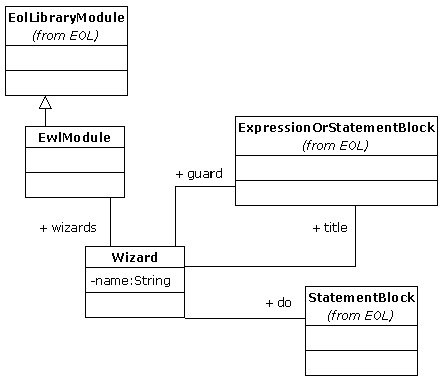
\includegraphics{images/EwlAbstractSyntax.png}
	\caption{EWL Abstract Syntax}
	\label{fig:EwlAbstractSyntax}
\end{figure}

\clearpage

\section{Concrete Syntax}

Listing \ref{lst:EwlConcreteSyntax} presents the concrete syntax of EWL wizards.

\begin{lstlisting}[caption=Concrete syntax of EWL wizards, label=lst:EwlConcreteSyntax, language=EWL]
wizard <name> {
	(guard (:expression)|({statementBlock}))?
	(title (:expression)|({statementBlock}))?
	do {
		statementBlock
	}
}
\end{lstlisting}

\section{Execution Semantics}
The process of executing EWL wizards is inherently user-driven and as such it depends on the environment in which they are used. In general, each time the selection of model elements changes (i.e. the user selects or deselects a model element in the modelling tool), the guards of all wizards are evaluated. If the guard of a wizard is satisfied, the \emph{title} part is also evaluated and the wizard is added to a list of \textit{applicable} wizards. Then, the user can select a wizard and execute its \emph{do} part to perform the intended transformation.

In EWL, variables defined and initialized in the \emph{guard} part of the wizard can be accessed both by the \emph{title} and the \emph{do} parts. In this way, results of calculations performed in the \emph{guard} part can be re-used, instead of re-calculated in the subsequent parts.  The practicality of this approach is discussed in more detail in the examples that follow. Also, the execution of the \emph{do} part of each wizard is performed in a transactional mode by exploiting the transaction capabilities of the underlying model connectivity framework, so that possible logical errors in the \emph{do} part of a wizard do not leave the edited model in an inconsistent state. 

\section{Examples}
\label{sec:EwlExamples}

This section presents three concrete examples of EWL wizards for refactoring UML 1.4 models. The aim of this section is not to provide complete implementations that address all the sub-cases of each scenario but to provide enhanced understanding of the concrete syntax, the features and the capabilities of EWL to the reader. Moreover, it should be stressed again that although the examples in this section are based on UML models, by building on Epsilon, EWL can be used to capture wizards for diverse modelling languages and technologies.

\subsubsection{Converting a Class into a Singleton}
\label{sec:ClassToSingleton}

The singleton pattern \cite{Larman} is applied when there is a class for which only one instance can exist at a time. In terms of UML, a singleton is a class stereotyped with the $<<singleton>>$ stereotype, and it defines a static attribute named \emph{instance} which holds the value of the unique instance. It also defines a static \emph{getInstance()} operation that returns that unique instance. Wizard \emph{ClassToSingleton}, presented in Listing \ref{lst:ClassToSingleton}, simplifies the process of converting a class into a singleton by adding the proper stereotype, attribute and operation to it automatically.

\begin{lstlisting}[
	basicstyle=\ttfamily\footnotesize, 
	flexiblecolumns=true,
	numbers=none,
	nolol=true,
	caption=Implementation of the ClassToSingleton Wizard, 
	label=lst:ClassToSingleton,
	numbers=left,
	language=EWL,
	tabsize=2
]
wizard ClassToSingleton {
	
	// The wizard applies when a class is selected
	guard : self.isTypeOf(Class)
	
	title : "Convert " + self.name + " to a singleton"
	
	do {
		// Create the getInstance() operation 
		var gi : new Operation; 
		gi.owner = self; 
		gi.name = "getInstance"; 
		gi.visibility = VisibilityKind#vk_public; 
		gi.ownerScope = ScopeKind#sk_classifier; 
		
		// Create the return parameter of the operation 
		var ret : new Parameter; 
		ret.type = self; 
		ret.kind = ParameterDirectionKind#pdk_return; 
		gi.parameter = Sequence{ret}; 
		
		// Create the instance field 
		var ins : new Attribute; 
		ins.name = "instance"; 
		ins.type = self; 
		ins.visibility = VisibilityKind#vk_private; 
		ins.ownerScope = ScopeKind#sk_classifier; 
		ins.owner = self; 
		
		// Attach the <<singleton>> stereotype 
		self.attachStereotype("singleton");
	}
}

// Attaches a stereotype with the specified name
// to the Model Element on which it is invoked
operation ModelElement attachStereotype(name : String) {
		var stereotype : Stereotype;
		
		// Try to find an existing stereotype with this name
		stereotype = Stereotype.allInstances.selectOne(s|s.name = name);
		
		// If there is no existing stereotype
		// with that name, create one
		if (not stereotype.isDefined()){
			stereotype = Stereotype.createInstance();
			stereotype.name = name;
			stereotype.namespace = self.namespace;
		}
		
		// Attach the stereotype to the model element
		self.stereotype.add(stereotype);
}
\end{lstlisting}

The \emph{guard} part of the wizard specifies that it is only applicable when the selection is a single UML class. The \emph{title} part specifies a context-aware title that informs the user of the functionality of the wizard and the \emph{do} part implements the functionality by adding the \emph{getInstance} operation (lines 10-14), the \emph{instance} attribute (lines 23-28) and the $<<singleton>>$ stereotype (line 31). 

The stereotype is added via a call to the \emph{attachStereotype()} operation. Attaching a stereotype is a very common action when refactoring UML models, particularly where UML profiles are involved, and therefore to avoid duplication, this reusable operation that checks for an existing stereotype, creates it if it does not already exists, and attaches it to the model element on which it is invoked has been specified.

An extended version of this wizard could also check for existing association ends that link to the class and for which the upper-bound of their multiplicity is greater than one and either disallow the wizard from executing on such classes (in the $guard$ part) or update the upper-bound of their multiplicities to one (in the $do$ part). However, the aim of this section is not to implement complete wizards that address all sub-cases but to provide a better  understanding of the concrete syntax and the features of EWL. This principle also applies to the examples presented in the sequel.
\subsubsection{Renaming a Class}
\label{sec:RenameClass}

The most widely used convention for naming attributes and association ends of a given class is to use a lower-case version of the name of the class as the name of the attribute or the association end. For instance, the two ends of a one-to-many association that links classes \texttt{Book} and \texttt{Chapter} are most likely to be named \texttt{book} and \texttt{chapters} respectively. When renaming a class (e.g. from \texttt{Chapter} to \texttt{Section}) the user must then manually traverse the model to find all attributes and association ends of this type and update their names (i.e. from \texttt{chapter} or \texttt{bookChapter} to \texttt{section} and \texttt{bookSection} respectively). This can be a daunting process especially in the context of large models. Wizard \texttt{RenameClass} presented in Listing \ref{lst:RenameClass} automates this process.

\begin{lstlisting}[
	basicstyle=\ttfamily\footnotesize, 
	flexiblecolumns=true, 
	numbers=none, 
	nolol=true, 
	caption=Implementation of the RenameClass Wizard,
	label=lst:RenameClass, 
	numbers=left, 
	language=EWL, 
	tabsize=2
]
wizard RenameClass {
	
	// The wizard applies when a Class is selected
	guard : self.isKindOf(Class)
	
	title : "Rename class " + self.name
	
	do {
		var newName : String;
		
		// Prompt the user for the new name of the class
		newName = UserInput.prompt("New name for class " + self.name);
		if (newName.isDefined()) {
			var affectedElements : Sequence;
			
			// Collect the AssociationEnds and Attributes
			// that are affected by the rename
			affectedElements.addAll(
				AssociationEnd.allInstances.select(ae|ae.participant=self));
			affectedElements.addAll(
				Attribute.allInstances.select(a|a.type = self));
			
			var oldNameToLower : String;
			oldNameToLower = self.name.firstToLowerCase();
			var newNameToLower : String;
			newNameToLower = newName.firstToLowerCase();
			
			// Update the names of the affected AssociationEnds
			// and Attributes
			for (ae in affectedElements) {
					ae.replaceInName(oldNameToLower, newNameToLower);
					ae.replaceInName(self.name, newName);
			}
			self.name = newName;
		}
	}
	
}

// Renames the ModelElement on which it is invoked
operation ModelElement replaceInName
	(oldString : String, newString : String) {
	
	if (oldString.isSubstringOf(self.name)) {
		// Calculate the new name
		var newName : String;
		newName = self.name.replace(oldString, newString);
		
		// Prompt the user for confirmation of the rename
		if (UserInput.confirm
			("Rename " + self.name + " to " + newName + "?")) {
			// Perform the rename
			self.name = newName;
		}
	}
}
\end{lstlisting}
%\vspace{-8pt}
As with the \texttt{ClassToSingleton} wizard, the \texttt{guard} part of \texttt{RenameClass} specifies that the wizard is applicable only when the selection is a simple class and the \emph{title} provides a context-aware description of the functionality of the wizard. 

As discussed in Section \ref{sec:ModelTransformationInTheSmall}, the information provided by the selected class itself does not suffice in the case of renaming since the new name of the class is not specified anywhere in the existing model. In EWL, and in all languages that build on EOL, user input can be obtained using the built-in \texttt{UserInput} facility. Thus, in line 12 the user is prompted for the new name of the class using the \texttt{UserInput.prompt()} operation. Then, all the association ends and attributes that refer to the class are collected in the \texttt{affectedElements} sequence (lines 14-21). Using the \texttt{replaceInName} operation (lines 31 and 32), the name of each one is examined for a substring of the upper-case or the lower-case version of the old name of the class. In case the check returns true, the user is prompted to confirm (line 48) that the feature needs to be renamed. This further highlights the importance of user input for implementing update transformations with fine-grained user control. 
\subsubsection{Moving Model Elements into a Different Package}
\label{sec:MoveToPackage}

A common refactoring when modelling in UML is to move model elements, particularly Classes, between different packages. When moving a pair of classes from one package to another, the associations that connect them must also be moved in the target package. To automate this process, Listing \ref{lst:MoveToPackage} presents the \texttt{MoveToPackage} wizard.

\begin{lstlisting}[
	basicstyle=\ttfamily\footnotesize, 
	flexiblecolumns=true, 
	numbers=none, 
	nolol=true, 
	caption=Implementation of the MoveToPackage Wizard, 
	label=lst:MoveToPackage, 
	numbers=left, 
	language=EWL, 
	tabsize=2
]
wizard MoveToPackage {
	
	// The wizard applies when a Collection of
	// elements, including at least one Package
	// is selected
	guard { 
		var moveTo : Package;
		if (self.isKindOf(Collection)) {
			moveTo = self.select(e|e.isKindOf(Package)).last();
		}
		return moveTo.isDefined();
	}
	
	title : "Move " + (self.size()-1) + " elements to " + moveTo.name
	
	do {
		// Move the selected Model Elements to the
		// target package
		for (me in self.excluding(moveTo)) {
			me.namespace = moveTo;
		}
		
		// Move the Associations connecting any
		// selected Classes to the target package
		for (a in Association.allInstances) {
			if (a.connection.forAll(c|self.includes(c.participant))){
				a.namespace = moveTo;
			}
		}
	}
	
}
\end{lstlisting}

The wizard applies when more than one element is selected and at least one of the elements is a \emph{Package}. If more than one package is selected, the last one is considered as the target package to which the rest of the selected elements will be moved. This is specified in the \emph{guard} part of the wizard.

To reduce user confusion in identifying the package to which the elements will be moved, the name of the target package appears in the title of the wizard. This example shows the importance of the decision to express the title as a dynamically calculated expression (as opposed to a static string). It is worth noting that in the \emph{title} part of the wizard (line 14), the \emph{moveTo} variable declared in the \emph{guard} (line 7) is referenced. Through experimenting with a number of wizards, it has been noticed that in complex wizards repeated calculations need to be performed in the \emph{guard}, \emph{title} and \emph{do} parts of the wizard. To eliminate this duplication, the scope of variables defined in the \emph{guard} part has been extended so that they are also accessible from the \emph{title} and \emph{do} part of the wizard.


\section{Summary}

This section has presented the Epsilon Wizard Language (EWL), a language for specifying and executing update transformations in the small on models of diverse metamodels. EWL provides a textual concrete syntax tailored to the task and features such as dynamically calculated wizard titles, transactional execution of the \emph{do} parts of wizards and user interaction.

\chapter{The Epsilon Generation Language (EGL)}
\label{sec:EGL}

EGL provides a language for M2T in the large.   EGL is a model-driven
template-based code generator, built atop Epsilon, and re-using all
of EOL. In this section, we discuss the  design of EGL and its
construction from existing Epsilon tools.

\section{Abstract Syntax}
Figure \ref{fig:abstractsyntax} depicts the abstract syntax of EGL's core functionality.

\begin{figure}[htbp]
  \begin{center}
    \leavevmode
    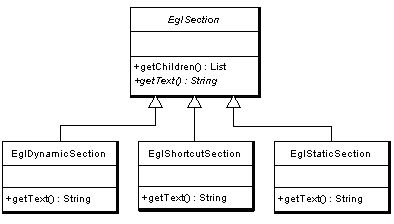
\includegraphics[scale=0.80]{images/EglAbstractSyntax.png}
  \end{center}
  \caption{The abstract syntax of EGL's core.}
  \label{fig:abstractsyntax}
\end{figure}

In common with other template-based code generators, EGL defines
\emph{sections}, from which templates may be constructed. Static
sections delimit sections whose contents appear verbatim in the
generated text. Dynamic sections contain executable code that can be
used to control the generated text.

In its dynamic sections, EGL re-uses EOL's mechanisms for structuring
program control flow, performing model inspection and navigation, and
defining custom operations.  EGL provides an EOL object, \verb|out|,
for use within dynamic sections.  This can be used to perform
operations on the generated text, such as appending and removing
strings and specifying the type of text to be generated.

EGL also provides syntax for defining \textit{dynamic output}
sections, which provide a convenient shorthand for outputting text
from within dynamic sections. Similar syntax is often provided by
template-based code generators.

\section{Concrete Syntax}
\label{concretesyntax}

The concrete syntax of EGL mirrors the style of other
template-based code generation languages. The tag pair \verb|[% %]| is
used to delimit a dynamic section. Any text not enclosed in such a tag
pair is contained in a static section. Listing
\ref{lst:basic} illustrates the use of dynamic and static sections to
form a basic EGL template.

\begin{lstlisting}[basicstyle=\ttfamily\footnotesize, tabsize=2, flexiblecolumns=true, caption=A basic EGL template., label=lst:basic]
[% for (i in Sequence{1..5}) { %]
i is [%=i%]
[% } %]
\end{lstlisting}

The \emph{[\%=expr\%]} construct is shorthand for \emph{[\%
  out.print(expr); \%]}, which appends \emph{expr} to the output
generated by the transformation. Note that the \verb|out| keyword also
provides \emph{println(Object)} and \emph{chop(Integer)} methods, which
can be used to construct text with linefeeds, and to remove the
specified number of characters from the end of the generated text.

EGL exploits EOL's model querying capabilities to output text from
models specified as input to transformations. For example, the EGL
template depicted in Listing \ref{lst:oo} may be used to generate text
from a model that conforms to a metamodel that describes an
object-oriented system.

\begin{lstlisting}[basicstyle=\ttfamily\footnotesize, tabsize=2, flexiblecolumns=true, caption=Generating the name of each Class contained in an input model., label=lst:oo]
[% for (class in Class.allInstances) { %]
[%=class.name%]
[% } %]
\end{lstlisting}

\section{Parsing and Preprocessing}
EGL provides a parser which generates an abstract syntax tree comprising static, dynamic and dynamic output nodes for a given template. A preprocessor then translates each section into corresponding EOL: static and dynamic output sections generate \verb|out.print()| statements. Dynamic sections are already specified in EOL, and require no translation.

Consider the EGL depicted in Listing \ref{lst:basic}.  The
preprocessor produces the EOL
shown in Listing
\ref{lst:preprocessor-eol} -- the \verb|[% %]| and \verb|[%=  %]| tag pairs have been removed, and the text to be output is translated into \verb|out.print()| statements.

\begin{lstlisting}[basicstyle=\ttfamily\footnotesize, tabsize=2, flexiblecolumns=true, caption=Resulting EOL generated by the preprocessor., label=lst:preprocessor-eol]
for (i in Sequence{1..5}) {
   out.print(`i is ');
   out.print(i);
   out.print(`\r\n');
}
\end{lstlisting}

When comparing Listings \ref{lst:basic} and \ref{lst:preprocessor-eol}, it can be seen that the template-based syntax is more concise, while the preprocessed syntax is arguably more readable. For templates where there is more dynamic than static text, such as the one depicted in Listing \ref{lst:basic}, a template-based syntax is often less readable. However, this loss of readability is somewhat mitigated by EGL's developer tools, which are discussed in Section \ref{Tool Support}. By contrast, for templates that exhibit more static than dynamic text, a template-based syntax is often more readable than its preprocessed equivalent.

\section{Deriving EGL from EOL}

In designing functionality specific to M2T transformation, one option
was to 
enrich the existing EOL syntax with  keywords such as \emph{print}, \emph{contentType} 
and \emph{merge}.  However, EOL underpins all Epsilon
languages, and the additional keywords were needed only for M2T.
Furthermore, the refactorings needed to support the new keywords
affect many components -- the lexer, parser, execution context and
execution engine -- complicating maintenance and use by other developers.
Instead, we define a minimal syntax for EGL, allowing easy
implementation of an EGL execution engine as a simple preprocessor for EOL. 
 

The EGL execution engine augments the default context used by EOL
during execution with two read-only, global variables: \emph{out}
(Section \ref{concretesyntax}) and \emph{TemplateFactory} (Section
\ref{Co-ordination}). The \emph{out} object defines methods for
performing operations specific to M2T translation, and the
\emph{TemplateFactory} object provides methods for loading other
templates. The implementation for the latter was extended, late in the
EGL development, to provide support for accessing templates from a
file-system -- a trivial extension that caused no migration problems
for existing EGL templates, due to the way in which EGL extends EOL.

\section{Co-ordination}
\label{Co-ordination}
In the large, M2T transformations need to be able to not only generate
text, but also files, which are then used downstream as development
artefacts.  An M2T tool must provide the language constructs for
producing files and manipulating the local file system.  Often, this
requires that the destination, as well as the contents, be dynamically
defined at a transformation's execution time.

The EGL co-ordination engine supplies mechanisms for generating text
directly to files.  The design encourages decoupling of generated text
from output destinations. The \emph{Template} data-type is provided to
allow nested execution of M2T transformations, and operations on
instances of this data-type facilitate the generation of text directly
to file. A factory object, \emph{TemplateFactory}, is provided to
simplify the creation of \emph{Template} objects.  In Listing
\ref{lst:co-ordination}, these objects are used in an EGL template
that loads the the EGL template in Listing \ref{lst:oo} from the file,
ClassNames.egl, and writes out to disk the text generated by executing
ClassNames.egl.

\begin{lstlisting}[basicstyle=\ttfamily\footnotesize, tabsize=2, flexiblecolumns=true, caption=Storing the name of each Class to disk., label=lst:co-ordination]
[%
  var t : Template := TemplateFactory.load(`ClassNames.egl');
  t.process();
  t.generate(`Output.txt');
%]
\end{lstlisting}

This approach to co-ordination allows EGL to be used to generate one
or more files from a single input model. Moreover, EGL's co-ordination
engine facilitates the specification of platform-specific details (the
destination of any files being generated) separately from the
platform-independent details (the contents of any files being
generated).

\section{Merge Engine}
EGL provides language constructs that allow M2T transformations to
designate regions of generated text as \textit{protected}. The
contents of protected regions are preserved every time a M2T
transformation generates text to the same destination.

Protected regions are specified by the \emph{preserve(String, String,
  String, Boolean, String)} method on the \verb|out| keyword. The first two parameters define the comment delimiters
of the target language. The other parameters provide the name,
enable-state and content of the protected region, as
illustrated in Listing \ref{lst:preserve}.

\begin{lstlisting}[basicstyle=\ttfamily\footnotesize, tabsize=2, flexiblecolumns=true, caption=Protected region declaration using the preserve method., label=lst:preserve]
[%=out.preserve(`/*', `*/', `anId', true,
                `System.out.println(foo);')
%]
\end{lstlisting}

A protected region declaration may have many lines, and use many EGL
variables in the contents definition.  To enhance readability, EGL
provides two additional methods on the \verb|out| keyword:
\emph{startPreserve(String, String, String, Boolean)} and
\verb|stopPreserve|.  Listing \ref{lst:startpreserve} uses these to
generate a protected region equivalent to that in Listing
\ref{lst:preserve}.

\begin{lstlisting}[basicstyle=\ttfamily\footnotesize, tabsize=2, flexiblecolumns=true, caption=Protected region declaration., label=lst:startpreserve]
[%=out.startPreserve(`/*', `*/', `anId', true)%]
System.out.println(foo);
[%=out.stopPreserve()%]
\end{lstlisting}

Because an EGL template may contain many protected regions, EGL also
provides a separate method to set the target language generated by the
current template, \emph{setContentType(String)}. By default, EGL recognises Java, HTML, Visual Basic,
Perl and EGL as valid content types. An alternative configuration file
can be used to specify further content
types. Following a call to \verb|setContentType|, the first two
arguments to the \verb|preserve| and \verb|startPreserve| methods can
be omitted, as shown in Listing \ref{lst:contenttype}.

\begin{lstlisting}[basicstyle=\ttfamily\footnotesize, tabsize=2, flexiblecolumns=true, caption=Setting the content type., label=lst:contenttype]
[% out.setContentType(`Java'); %]
[%=out.preserve(`anId', true, `System.out.println(foo);')%]
\end{lstlisting}

Because some languages define more than one style of comment
delimiter, EGL allows mixed use of  the styles for \verb|preserve| and
\verb|startPreserve| methods.

Once a content type has been specified, a protected region may be declared entirely from a static section, using the syntax  in Listing \ref{lst:manualpr}.

\begin{lstlisting}[basicstyle=\ttfamily\footnotesize, tabsize=2, flexiblecolumns=true, caption=Declaring a protected region from within a static section., label=lst:manualpr]
[% out.setContentType(`Java'); %]
// protected region anId [on|off] begin
System.out.println(foo);
// protected region anId end
\end{lstlisting}

When a template that defines one or more protected regions is
processed by the EGL execution engine, the target output destinations
are interrogated and existing contents of any protected regions are
preserved. If either the output generated by from the template or the
existing contents of the target output destination contains protected
regions, a merging process is invoked. Table \ref{tab:merging} shows
the default behaviour of EGL's merge engine.

\begin{table}[htbp]
  \begin{center}
  \begin{tabular}{|l|l|l|}
  \hline
  \multicolumn{2}{|l|}{\textbf{Protected Region Status}} & \multirow{2}{*}{\textbf{Contents taken from}} \\
  \textbf{Generated} & \textbf{Existing} & \\
  \hline
  On & On     & Existing  \\
  On & Off    & Generated \\
  On & Absent & Generated \\
  \hline
  Off & On     & Existing  \\
  Off & Off    & Generated \\
  Off & Absent & Generated \\
  \hline
  Absent & On  & Neither (causes a warning) \\
  Absent & Off & Neither (causes a warning) \\
  \hline
  \end{tabular}
  \end{center}
\caption{EGL's default merging behaviour.}
\label{tab:merging}
\end{table}

\section{Readability and traceability} 
Conscientious developers apply various \emph{conventions} to produce
readable code.  EGL encourages template developers to prioritise the
readability of templates over the text that they generate. EGL provides a number of text post-processors -- or
\textit{beautifiers} -- that can be executed on output of
transformations to improve readability.  Currently, beautifiers are
invoked via Epsilon's extensions to Apache Ant, an
XML-based build tool for Java.

EGL also provides a traceability API, as a debugging aid, and to
support auditing of the M2T transformation process.  This API
facilitates exploration of the templates executed, files affected and
protected regions processed during a transformation.  Figure
\ref{fig:traceability} shows sample output from the traceability API
after execution of an EGL M2T transformation to generate Java
code from an instance of an OO metamodel.

The beautification interface is minimal, in order to allow re-use of existing 
code formatting algorithms. Consequently, there is presently no traceability support 
for beautified text. However, due to the coarse-grained approach employed by 
EGL's traceability API, this has little impact: Clicking on a beautified protected 
region in the traceability view might not highlight the correct line in the editor.

\begin{figure}[htbp]
  \begin{center}
    \leavevmode
    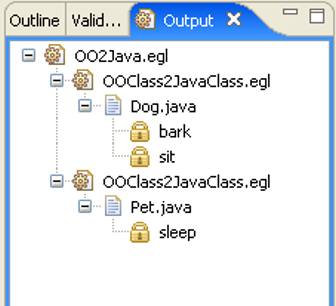
\includegraphics[scale=0.6]{images/TraceView}
  \end{center}
  \caption{Sample output from the traceability API.}
  \label{fig:traceability}
\end{figure}

\subsection{Tool Support}
\label{Tool Support}
The Epsilon platform provides development tools for the Eclipse
development environment. Re-use of Eclipse APIs allows
Epsilon's development tooling to incorporate a large number of
features with minimal effort. Furthermore, the flexibility of the
plug-in architecture of Eclipse enhances modular authoring of
development tools for Epsilon.

In addition to the traceability view shown in Figure
\ref{fig:traceability}, EGL includes an Eclipse editor and an outline
view. In order to aid template readability, these tools provide syntax 
highlighting and a structural overview for EGL templates, respectively. Through its 
integration in the Epsilon perspective, EGL provides an Eclipse workbench 
configuration that is tailored for use with Epsilon's development tools.

%\begin{figure}[htbp]
%  \begin{center}
%    \leavevmode
%    \includegraphics[scale=0.66]{EglWorkspace.png}
%  \end{center}
%  \caption{The EGL editor and outline view.}
%  \label{fig:editorandview}
%\end{figure}

EGL, like other Epsilon languages, provides an Apache ANT
task definition, to facilitate invocation of model-management activies
from within a build script.

\chapter{The Epsilon Comparison Language (ECL)}
\label{sec:ECL}

Model comparison is the task of identifying \emph{matching} elements between models. In general, \emph{matching} elements are elements that are involved in a relationship of interest. For example, before merging homogeneous models, it is essential to identify overlapping (common) elements so that they do not appear in duplicate in the merged model. Similarly, in heterogeneous model merging, it is a prerequisite to identify the elements on which the two models will be merged. Finally, in transformation testing, matching elements are pairs consisting of elements in the input model and their generated counterparts in the output model.

The aim of the Epsilon Comparison Language (ECL) is to enable users to specify comparison algorithms in a rule-based manner to identify pairs of matching elements between two models of potentially different metamodels and modelling technologies. In this section, the abstract and concrete syntax, as well as the execution semantics of the language, are discussed in detail.

%A comparison algorithm separates the model elements of the involved models into two categories: those that have matching elements in the opposite model and those that do not. Moreover, as the algorithm does not necessarily attempt to find matching elements for all the model elements of the involved models, the classification can be further refined to the following:
%
%\begin{enumerate}
%	\item Elements for which matching elements exist in the opposite model
%	\item Elements for which matching elements do not exist in the opposite model
%	\begin{enumerate}
%	\item Elements for which matching has been attempted but no matching elements has been found
%	\item Elements for which no matching has been attempted
%	\end{enumerate}
%\end{enumerate}

\section{Abstract Syntax}

In ECL, comparison specifications are organized in modules (\emph{EcLModule}). As illustrated in Figure \ref{fig:ECL}, EclModule extends EOLLibraryModule which means that it can contain user-defined operations and import other library modules and ECL modules. Apart from operations, an ECL module contains a set of match-rules (\emph{MatchRule}) and a set of \emph{pre} and \emph{post} blocks.

\emph{MatchRules} enable users to perform comparison of model elements at a high level of abstraction. Each match-rule declares a name, and two parameters (\emph{leftParameter} and \emph{rightParameter}) that specify the types of elements it can compare. It also optionally defines a number of rules it inherits (\emph{extends}) and if it is \emph{abstract}, \emph{lazy} and/or \emph{greedy}. The semantics of the latter are discussed shortly.

\begin{landscape}
\begin{figure}
	\centering
		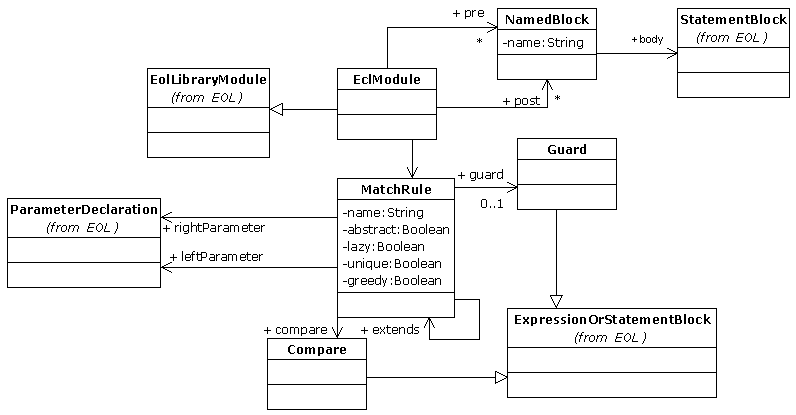
\includegraphics{images/EclAbstractSyntax.png}
	\caption{ECL Abstract Syntax}
	\label{fig:ECL}
\end{figure}
\end{landscape}

A match rule has three parts. The \emph{guard} part is an EOL expression or statement block that further limits the applicability of the rule to an even narrower range of elements than that specified by the \emph{left} and \emph{right} parameters. The \emph{compare} part is an EOL expression or statement block that is responsible for comparing a pair of elements and deciding if they match or not. Finally, the \emph{do} part is an EOL expression or block that is executed if the \emph{compare} part returns true to perform any additional actions required.

\emph{Pre} and \emph{Post} blocks are named blocks of EOL statements which as discussed in the sequel are executed before and after the match-rules have been executed respectively.

\section{Concrete Syntax}

The concrete syntax of a match-rule is displayed in Listing \ref{lst:MatchRuleConcreteSyntax}.

\begin{lstlisting}[basicstyle=\ttfamily\footnotesize, flexiblecolumns=true, numbers=none, nolol=true, caption=Concrete Syntax of a MatchRule, label=lst:MatchRuleConcreteSyntax, language=ECL, numbers=left, tabsize=2]

(@lazy)?
(@greedy)?
(@abstract)? 
rule <name> 
	match <leftParameterName>:<leftParameterType>
	with <rightParameterName>:<rightParameterType>
	(extends (<ruleName>,)*<ruleName>)? {
	
	(guard (:expression)|({statementBlock}))?
	
	compare (:expression)|({statementBlock})
	
	(do {statementBlock})?
	
}
\end{lstlisting}

\emph{Pre} and \emph{post} blocks have a simple syntax that, as presented in Listing \ref{lst:EclPrePostConcreteSyntax}, consists of the identifier (\emph{pre} or \emph{post}), an optional name and the set of statements to be executed enclosed in curly braces.

\begin{lstlisting}[basicstyle=\ttfamily\footnotesize, flexiblecolumns=true, numbers=none, nolol=true, caption=Concrete Syntax of Pre and Post blocks, label=lst:EclPrePostConcreteSyntax, language=ECL, numbers=left, tabsize=2]
(pre|post) <name> {
	statement+
}
\end{lstlisting}

\section{Execution Semantics}

\subsection{Rule and Block Overriding}

An ECL module can import a number of other ECL modules. In such a case, the importing ECL module inherits all the rules and pre/post blocks specified in the modules it imports (recursively). If the module specifies a rule or a pre/post block with the same name, the local rule/block overrides the imported one respectively.

\subsection{Comparison Outcome}

As illustrated in Figure \ref{fig:ECLRuntime}, the result of comparing two models with ECL is a trace (\emph{MatchTrace}) that consists of a number of matches (\emph{Match}). Each match holds a reference to the objects from the two models that have been compared (\emph{left} and \emph{right}), a boolean value that indicates if they have been found to be \emph{matching} or not, a reference to the \emph{rule} that has made the decision, and a Map (\emph{info}) that is used to hold any additional information required by the user. During the matching process, a second, temporary, match trace is also used to detect and resolve cyclic invocation of match-rules as discussed in the sequel.

\begin{figure}
	\centering
		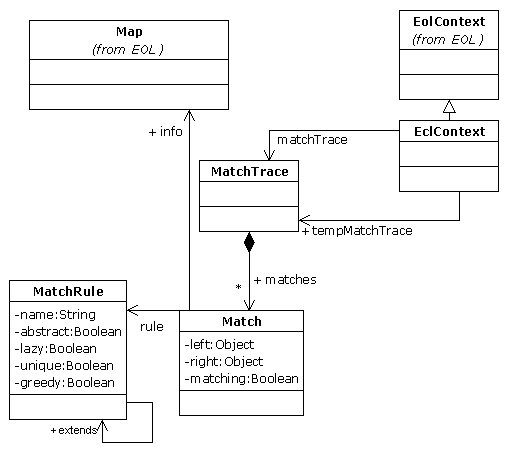
\includegraphics{images/ECLRuntime.png}
	\caption{ECL Match Trace}
	\label{fig:ECLRuntime}
\end{figure}

\subsection{Rule Execution Scheduling}

Non-abstract, non-lazy match-rules are evaluated automatically by the execution engine in a top-down fashion - with respect to their order of appearance - in two passes. In the first pass, each rule is evaluated for all the pairs of instances in the two models that have a type-of relationship with the types specified by the \emph{leftParameter} and \emph{rightParameter} of the rule. In the second pass, each rule that is marked as \emph{greedy} is executed for all pairs that have not been compared in the first pass, and which have a kind-of relationship with the types specified by the rule. In both passes, to evaluate the compare part of the rule, the guard must be satisfied.

Before the compare part of a rule is executed, the compare parts of all of the rules it extends (super-rules) must be executed (recursively). Before executing the compare part of a super-rule, the engine verifies that the super-rule is actually applicable to the elements under comparison by checking for type conformance and evaluating the guard part of the super-rule.

If the compare part of a rule evaluates to true, the optional do part is executed. In the do part the user can specify any actions that need to be performed for the identified matching elements, such as to populate the \emph{info} map of the established \emph{match} with additional information. Finally, a new match is added to the match trace that has its \emph{matching} property set to the logical conjunction of the results of the evaluation of the compare parts of the rule and its super-rules.

\subsection{The \emph{matches()} built-in operation}

To refrain from performing duplicate comparisons and to de-couple match-rules from each other, ECL provides the built-in \emph{matches(opposite : Any)} operation for model elements and collections. When the \emph{matches()} operation is invoked on a pair of objects, it queries the main and temporary match-traces to discover if the two elements have already been matched and if so it returns the cached result of the comparison. Otherwise, it attempts to find an appropriate match rule to compare the two elements and if such a rule is found, it returns the result of the comparison, otherwise it returns false. Unlike the top-level execution scheme, the \emph{matches()} operation invokes both \emph{lazy} and \emph{non-lazy} rules.

In addition to objects, the \emph{matches} operations can also be invoked to match pairs of collections of the same type (e.g. a Sequence against a Sequence). When invoked on ordered collections (i.e. \emph{Sequence} and \emph{OrderedSet}), it examines if the collections have the same size and each item of the source collection matches with the item of the same index in the target collection. Finally, when invoked on unordered collections (i.e. \emph{Bag} and \emph{Set}), it examines if for each item in the source collection, there is a matching item in the target collection irrespective of its index. Users can also override the built-in \emph{matches} operation using user-defined operations with the same name, as discussed in Section \ref{sec:Design.EOL.FeatureNavigation}, that loosen or strengthen the built-in semantics.

\subsection{Cyclic invocation of \emph{matches()}}

Providing the built-in \emph{matches} operation significantly simplifies comparison specifications. It also enhances decoupling between match-rules from each other as when a rule needs to compare two elements that are outside its scope, it does not need to know/specify which other rule can compare those elements explicitly.

On the other hand, it is possible - and quite common indeed - for two rules to implicitly invoke each other. For example consider the match rule of Listing \ref{lst:Tree2Tree} that attempts to match nodes of the simple Tree metamodel displayed in Figure \ref{fig:Tree}.

\begin{figure}
	\centering
		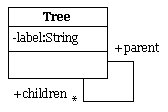
\includegraphics{images/metamodels/Tree.png}
	\caption{The Tree Metamodel}
	\label{fig:Tree}
\end{figure}

\begin{lstlisting}[basicstyle=\ttfamily\footnotesize, flexiblecolumns=true, numbers=none, nolol=true, caption=The Tree2Tree rule, label=lst:Tree2Tree, language=ECL, numbers=left, tabsize=2]
rule Tree2Tree 
	match l : T1!Tree
	with r : T2!Tree {
	
	compare : l.label = r.label and 
		l.parent.matches(r.parent) and
		l.children.matches(r.children)
}
\end{lstlisting}

The rule specifies that for two Tree nodes (\emph{l} and \emph{r}) to match, they should have the same label, belong to matching parents and have matching children. In the absence of a dedicated mechanism for cycle detection and resolution, the rule would end up in an infinite loop. To address this problem, ECL provides a temporary match-trace which is used to detect and resolve cyclic invocations of the \emph{match()} built-in operation.

As discussed above, a match is added to the primary match-trace as soon as the compare part of the rule has been executed to completion. By contrast, a temporary match (with its \emph{matching} property set to \emph{true}) is added to the temporary trace before the compare part is executed. In this way, any subsequent attempts to match the two elements from invoked rules will not re-invoke the rule. Finally, when a top-level rule returns, the temporary match trace is reset.

\section{Fuzzy and Dictionary-based String Matching}
\label{sec:FuzzyComparison}

In the example of Listing \ref{lst:Tree2Tree}, the rule specifies that to match, two trees must - among other criteria - have the same label. However, there are cases when a less-strict approach to matching string properties of model elements is desired. For instance, when comparing two UML models originating from different organizations, it is common to encounter ontologically equivalent classes which however have different names (e.g. Client and Customer). In this case, to achieve a more sound matching, the use of a dictionary or a lexical database (e.g. WordNet \cite{Wordnet}) is necessary. Alternatively, fuzzy string matching algorithms such as those presented in \cite{FuzzyStringMatching} can be used.

As several such tools and algorithms have been implemented in various programming languages, it is a sensible approach to reuse them instead of re-implementing them. For example, in Listing \ref{lst:FuzzyTree2Tree} a wrapper for the Simmetrics \cite{Simmetrics} fuzzy string comparison tool is used to compare the labels of the trees using the Levenshtein \cite{Levenshtein} algorithm. To achieve this, line 11 invokes the \emph{fuzzyMatch()} operation defined in lines 16-18 which uses the simmterics native tool (instantiated in lines 2-4) to match the two labels using their Levenshtein distance with a threshold of 0.5.

\begin{lstlisting}[basicstyle=\ttfamily\footnotesize, flexiblecolumns=true, numbers=none, nolol=true, caption=The FuzzyTree2Tree rule, label=lst:FuzzyTree2Tree, language=ECL, numbers=left, tabsize=2]
pre {
	var simmetrics = 
		new Native("org.epsilon.ecl.tools.
			textcomparison.simmetrics.SimMetricsTool"); 
}

rule FuzzyTree2Tree 
	match l : T1!Tree
	with r : T2!Tree {
	
	compare : l.label.fuzzyMatch(r.label) and 
		l.parent.matches(r.parent) and
		l.children.matches(r.children)
}

operation String fuzzyMatch(other : String) : Boolean {
	return simmetrics.similarity(self,other,"Levenshtein") > 0.5;
}\end{lstlisting}

\section{Interactive Matching}
\label{sec:InteractiveModelComparison}

Using the user interaction features discussed in Section \ref{sec:Design.EOL.UserInput} the comparison can become interactive by replacing the \emph{fuzzyMatch} operation of listing \ref{lst:FuzzyTree2Tree} with the one specified in Listing \ref{lst:InteractiveTree2TreeComparison}. The fuzzyMatch operation of Listing \ref{lst:InteractiveTree2TreeComparison}, performs the fuzzy string comparison and -- as the previous version -- if the result is greater than 0.5 it returns true. However, in this updated version if the result is lower than 0.5 but greater than 0.3, it prompts the user to confirm if the two strings match, and if it is lower than 0.3 it returns false.

\begin{lstlisting}[basicstyle=\ttfamily\footnotesize, flexiblecolumns=true, numbers=none, nolol=true, caption=An interactive version of the fuzzyMatch operation of Listing \ref{lst:FuzzyTree2Tree}, label=lst:InteractiveTree2TreeComparison, language=ECL, numbers=left, tabsize=2]
operation String fuzzyMatch(other : String) : Boolean {
	var similarity : Real;
	similarity = simmetrics.similarity(self,other,"Levenshtein");
	if (similarity > 0.5) {
		return true;
	}
	else if (similarity > 0.3) {
		return UserInput.confirm(self + " matches " + other + "?");
	}
	else {
		return false;
	}
}\end{lstlisting}

\section{Exploiting the Comparison Outcome}

Users can query and modify the match trace calculated during the comparison process in the post sections of the module or export it into another application or Epsilon program. For example, in a post section, the trace can be printed to the default output stream or serialized into a model of an arbitrary metamodel. In another use case, the trace may be exported to be used in the context of a validation module that will use the identified matches to evaluate inter-model constraints, or in a merging module that will use the matches to identify the elements on which the two models will be merged. The topic of interoperability - that includes importing and exporting objects - between modules expressed in different Epsilon languages is discussed in Chapter \ref{chp:Workflow}.

\chapter{The Epsilon Merging Language (EML)}
\label{sec:EML}

The aim of EML is to contribute model merging capabilities to Epsilon. More specifically, EML can be used to merge an arbitrary number of input models of potentially diverse metamodels and modelling technologies. This section provides a discussion on the motivation for implementing EML, its abstract and concrete syntax, as well as its execution semantics. It also provides two examples of merging homogeneous and heterogeneous models.

\section{Motivation}

A mechanism that enables automatically merging models on a set of established correspondences has a number of applications in a model driven engineering process. For instance, it can be used to unify two complementary, but potentially overlapping, models that describe different views of the same system. In another scenario, it can be used to merge a core model with an aspect model (potentially conforming to different metamodels), as discussed in \cite{MDAGuide} where a core \emph{Platform Independent Model (PIM)} is merged with a \emph{Platform Definition Model (PDM)}, that contributes platform-specific aspects, into a \emph{Platform Specific Model (PSM)}.

\subsection{Phases of Model Merging}

Existing research \cite{Pottinger2003,Batini1986} has demonstrated that model merging can be decomposed into four distinct phases: comparison, conformance checking, merging and reconciliation (or restructuring).

\paragraph{Comparison Phase} In the comparison phase, correspondences between equivalent elements of the source models are identified, so that such elements are not propagated in duplicate in the merged model.

%In \cite{ModelWeaver} the ModelWeaver, a generic framework for capturing different types of relationships, such as match relationships, between elements of different models is illustrated.  Matching pairs of elements can be defined graphically through a tree-based user interface and declared relationships can be stored in a separate \textit{weaving model}. Weaving models can be used later by other tools such as model transformation or model merging tools. While this is a flexible approach that promotes reuse, it does not scale well since manual definition of each matching pair is a labour intensive process.

%In \cite{Alanen2003}, matching is performed using persistent model-element identifiers (i.e. using the $xmi.id$ identifier). However, this only applies to comparison of models that are versions of a common ancestor. In \cite{Gray2005}, matching is performed by comparing the \textit{names} of the elements of the two models. Nevertheless, there are model elements that do not have a name (e.g. instances of the $Multiplicity$ UML metaclass) to compare.

\paragraph{Conformance Checking Phase} In this phase, elements that have been identified as matching in the previous phase are examined for conformance with each other. The purpose of this phase is to identify potential conflicts that would render merging infeasible. The majority of proposed approaches, such as \cite{Letkeman2005}, address conformance checking of models complying with the same metamodel. 
 
\paragraph{Merging Phase}
Several approaches have been proposed for the merging phase. In \cite{Pottinger2003,Melnik2003}, graph-based algorithms for merging models of the same metamodel are proposed. In \cite{Letkeman2005}, an interactive process for merging of UML 2.0 models is presented. There are at least two weaknesses in the methods proposed so far. First, they only address the issue of merging models of the same metamodel, and some of them address a specific metamodel indeed. Second, they use an inflexible merging algorithm and do not provide means for extending or customizing its logic.

\paragraph{Reconciliation and Restructuring Phase}
After the merging phase, the target model may contain inconsistencies that need fixing. In the final step of the process, such inconsistencies are removed and the model is \textit{polished} to acquire its final form. Although the need for a reconciliation phase is discussed in \cite{Batini1986,Melnik2003}, in the related literature the subject is not explicitly targeted.

\subsection{Relationship between Model Merging and Model Transformation}

A merging operation is a transformation in a general sense, since it transforms some input (source models) into some output (target models). However, as discussed throughout this section, a model merging facility has special requirements (support for comparison, conformance checking and merging pairs of input elements) that are not required for typical \textit{one-to-one} or \textit{one-to-many} transformations \cite{Czarnecki2003} and are therefore not supported by contemporary model transformation languages.

\section{Realizing a Model Merging Process with Epsilon}

The first two steps of the process described above can be realized with existing languages provided by Epsilon. As discussed in Section \ref{sec:ECL}, the comparison step can be realized with the Epsilon Comparison Language (ECL). Following that, the Epsilon Validation Language (EVL) can be used to validate the identified correspondences using the match trace calculated by ECL. The Epsilon Merging Language (EML) presented below provides support for the last two steps of the process (merging and reconciliation/restructuring).

\section{Abstract Syntax}

In EML, merging specifications are organized in modules (\emph{EmlModule}). As displayed in Figure \ref{fig:EmlAbstractSyntax}, \emph{EmlModule} inherits from \emph{EtlModule}.

\begin{sidewaysfigure}
  \centering
  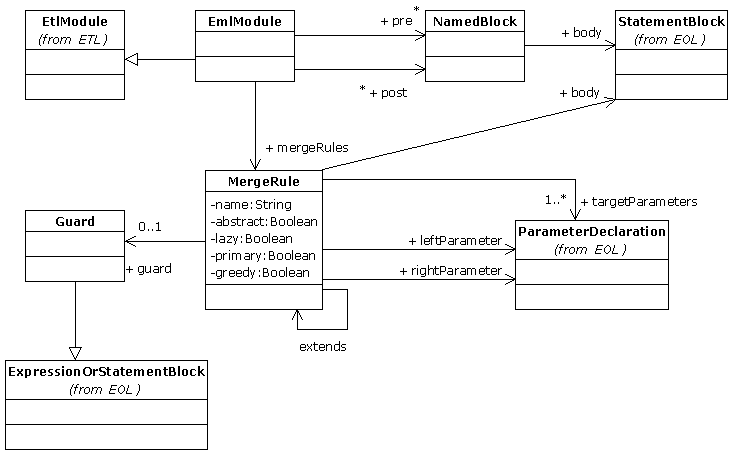
\includegraphics{images/EmlAbstractSyntax.png}
  \caption{The Abstract Syntax of EML}
  \label{fig:EmlAbstractSyntax}
\end{sidewaysfigure}

By extending \emph{EtlModule}, an EML module can contain a number of transformation rules and user-defined operations. An EML module can also contain one or more merge rules as well as a set of \emph{pre} and \emph{post} named EOL statement blocks. As usual, \emph{pre} and \emph{post} blocks will be run before and after all rules, respectively.

Each merge rule defines a name, a left, a right, and one or more target parameters. It can also extend one or more other merge rules and be defined as having one or more of the following properties: abstract, greedy, lazy and primary.

\section{Concrete Syntax}

Listing \ref{lst:EmlConcreteSyntax} demonstrates the concrete syntax of EML merge-rules.

\begin{lstlisting}[float=tbp, caption=Concrete syntax of an EML merge-rule, label=lst:EmlConcreteSyntax, language=EML]
(@abstract)?
(@lazy)?
(@primary)?
(@greedy)?
rule <name>
	merge <leftParameter>
	with <rightParameter>
	into (<targetParameter>(, <targetParameter>)*)?
	(extends <ruleName>(, <ruleName>)*)? {

	statementBlock
	
}
\end{lstlisting}

\emph{Pre} and \emph{post} blocks have a simple syntax that, as presented in Listing \ref{lst:EmlPrePostConcreteSyntax}, consists of the identifier (\emph{pre} or \emph{post}), an optional name and the set of statements to be executed enclosed in curly braces.

\begin{lstlisting}[float=tbp, caption=Concrete Syntax of Pre and Post blocks, label=lst:EmlPrePostConcreteSyntax, language=EML]
(pre|post) <name> {
	statement+
}
\end{lstlisting}

\section{Execution Semantics}

\subsection{Rule and Block Overriding}
An EML module can import a number of other EML and ETL modules. In this case, the importing EML module inherits all the rules and pre/post blocks specified in the modules it imports (recursively). If the module specifies a rule or a pre/post block with the same name, the local rule/block overrides the imported one respectively.

\subsection{Rule Scheduling}
When an EML module is executed, the \emph{pre} blocks are executed in the order in which they have been defined.

Following that, for each \emph{match} of the established \emph{matchTrace} the applicable non-abstract, non-lazy merge rules are executed. When all \emph{matches} have been merged, the transformation rules of the module are executed on all applicable elements - that have not been merged - in the models.

Finally, after all rules have been applied, the \emph{post} blocks of the module are executed.

\subsection{Rule Applicability}
By default, for a merge-rule to apply to a \emph{match}, the \emph{left} and \emph{right} elements of the match must have a \emph{type-of} relationship with the \emph{leftParameter} and \emph{rightParameter} of the rule respectively. This can be relaxed to a \emph{kind-of} relationship by specifying that the merge rule is \emph{greedy} (using the \emph{@greedy} annotation in terms of concrete syntax).

\subsection{Source Elements Resolution}

As with model transformation, in model merging it is often required to resolve the counterparts of an element of a source model into the target models. In EML, this is achieved by overloading the semantics of the \emph{equivalents()} and \emph{equivalent()} operations defined by ETL. In EML, in addition to inspecting the transformation trace and invoking any applicable transformation rules, the \emph{equivalents()} operation also examines the \emph{mergeTrace} (displayed in Figure \ref{fig:EmlRuntime}) that stores the results of the application of merge-rules and invokes any applicable (both lazy and non-lazy) rules.

Similarly to ETL, the order of the results of the \emph{equivalents()} operation respects the order of the (merge or transform) rules that have produced them. An exception to that occurs if one of the rules has been declared as primary, in which case its results are prepended to the list of elements returned by equivalent.

\begin{figure}
	\centering
		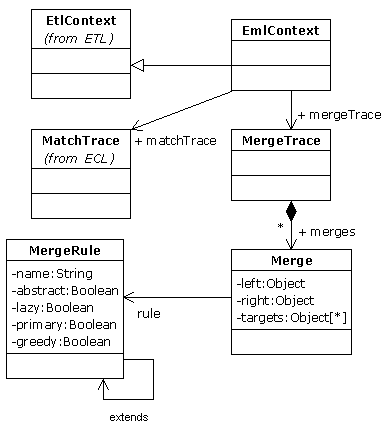
\includegraphics{images/EmlRuntime.png}
	\caption{The EML runtime}
	\label{fig:EmlRuntime}
\end{figure}

\section{Homogeneous Model Merging Example}

In this scenario, two models conforming to the Graph metamodel need to be merged. The first step is to compare the two graphs using the ECL module of Listing \ref{lst:CompareGraph}.

\begin{lstlisting}[float=tbp, caption=ECL module for comparing two instances of the Graph metamodel, label=lst:CompareGraph, language=ECL, tabsize=2]
rule MatchNodes /*@\label{line:MatchNodes}@*/
	match l : Left!Node
	with r : Right!Node {

	compare : l.label = r.label
}

rule MatchEdges /*@\label{line:MatchEdges}@*/
	match l : Left!Edge
	with r : Right!Edge {

	compare : l.source.matches(r.source)
		and l.target.matches(r.target)
}

rule MatchGraphs /*@\label{line:MatchGraphs}@*/
	match l : Left!Graph
	with r : Right!Graph {

	compare : true
}
\end{lstlisting}

The \emph{MatchNodes} rule in line \ref{line:MatchNodes} defines that two nodes match if they have the same label. The \emph{MatchEdges} rule in line \ref{line:MatchEdges} specifies that two edges match if both their source and target nodes match (regardless of whether the labels of the edges match or not as it is assumed that there can not be two distinct edges between the same nodes). Finally, since only one instance of Graph is expected to be in each model, the \emph{MatchGraphs} rule in line \ref{line:MatchGraphs} returns \emph{true} for any pair of Graphs\footnote{Both assumptions can be checked using EVL before matching/merging takes place but this is out of the scope of this example}.

Having established the necessary correspondences between matching elements of the two models, the EML specification of listing \ref{lst:MergeGraphs}.

\begin{lstlisting}[float=tbp, label=lst:MergeGraphs, caption=EML module for merging two instances of the Graph metamodel on the correspondences identified in Listing \ref{lst:CompareGraph} , language=EML]
import "Graphs.etl";

rule MergeGraphs /*@\label{line:MergeGraphs}@*/
	merge l : Left!Graph
	with r : Right!Graph
	into t : Target!Graph {
	
	t.label = l.label + " and " + r.label;
	
}

@abstract
rule MergeGraphElements /*@\label{line:MergeGraphElements}@*/
	merge l : Left!GraphElement
	with r : Right!GraphElement
	into t : Target!GraphElement {
	
	t.graph ::= l.graph;
	
}

rule MergeNodes /*@\label{line:MergeNodes}@*/
	merge l : Left!Node
	with r : Right!Node
	into t : Target!Node 
	extends GraphElements {
	
	t.label = "c_" + l.label;
	
}
rule MergeEdges /*@\label{line:MergeEdges}@*/
	merge l : Left!Edge
	with r : Right!Edge
	into t : Target!Edge 
	extends GraphElements {
	
	t.source ::= l.source;
	t.target ::= l.target;
	
}
\end{lstlisting}

In line \ref{line:MergeGraphs}, the \emph{MergeGraphs} merge rule specifies that two matching Graphs (\emph{l} and \emph{r}) are to be merged into one Graph \emph{t} in the target model that has as a label, the concatenation of the labels of the two input graphs separated using 'and'. The \emph{mergeNodes} rule In line \ref{line:MergeNodes} specifies that two matching Nodes are merged into a single Node in the target model. The label of the merged node is derived by concatenating the c (for common) static string with the label of the source Node from the left model. Similarly, the \emph{MergeEdges} rule specifies that two matching Edges are merged into a single Edge in the target model. The source and target nodes of the merged Edge are set to the equivalents (::=) of the source and target nodes of the edge from the left model.

To reduce duplication, the \emph{MergeNodes} and \emph{MergeEdges} rules extend the abstract \emph{MergeGraphElements} rule specified in line \ref{line:MergeGraphElements} which assigns the \emph{graph} property of the graph element to the equivalent of the left graph.

The rules displayed in Listing \ref{lst:MergeGraphs} address only the matching elements of the two models. To also copy the elements for which no equivalent has been found in the opposite model, the EML module imports the ETL module of Listing \ref{lst:CopyGraph}.

\begin{lstlisting}[float=tbp, caption=The Graphs.etl ETL transformation module, label=lst:CopyGraph, language=ETL]
rule TransformGraph 
	transform s : Source!Graph
	to t : Target!Graph {
	
	t.label = s.label;
	
}

@abstract
rule TransformGraphElement 
	transform s : Source!GraphElement
	to t : Target!GraphElement {
	
	t.graph ::= s.graph;
}

rule TransformNode /*@\label{line:TransformNode}@*/
	transform s : Source!Node
	to t : Target!Node 
	extends TransformGraphElement {
	
	t.label = s.graph.label + "_" + s.label;
}

rule TransformEdge 
	transform s : Source!Edge
	to t : Target!Edge 
	extends TransformGraphElement {
	
	t.source ::= s.source;
	t.target ::= s.target;	
} 
\end{lstlisting}

The rules of the ETL module apply to model elements of both the Left and the Right model as both have been aliased as Source. Of special interest is the TransformNode rule in line \ref{line:TransformNode} that specifies that non-matching nodes in the two input models will be transformed into nodes in the target model the labels of which will be a concatenation of their input graph and the label of their counterparts in the input models.

Executing the ECL and EML modules of Listings \ref{lst:CompareGraph} and \ref{lst:MergeGraphs} on the exemplar models displayed in Figures \ref{fig:LeftGraph} and \ref{fig:RightGraph} creates the target model of Figure \ref{fig:TargetGraph}.

\begin{figure}
	\centering
		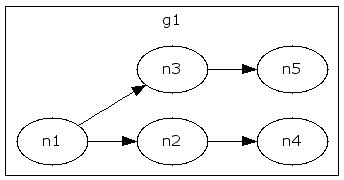
\includegraphics{images/LeftGraph.png}
	\caption{Left input model}
	\label{fig:LeftGraph}
\end{figure}


\begin{figure}
	\centering
		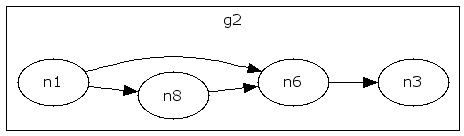
\includegraphics{images/RightGraph.png}
	\caption{Right input model}
	\label{fig:RightGraph}
\end{figure}


\begin{figure}
	\centering
		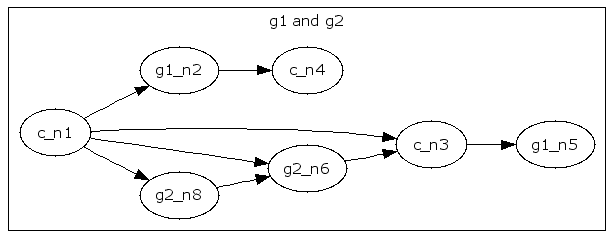
\includegraphics{images/MergedGraph.png}
	\caption{Target model derived by merging the models of Figures \ref{fig:LeftGraph} and \ref{fig:RightGraph}}
	\label{fig:TargetGraph}
\end{figure}

%!TEX root = ./EpsilonBook.tex

\chapter{Epsilon Flock for Model Migration}
\label{sec:Flock}

The aim of Epsilon Flock is to contribute \emph{model migration} capabilities to Epsilon. Model migration is the process of updating models in response to metamodel changes. This section discusses the motivation for implementing Flock, introduces its syntax and execution semantics, and demonstrates the use of Flock with an example.
Flock can be used to update models to a new version of their metamodel, or even to move from one modelling technology to another (e.g., from XML to EMF).

\section{Background and Motivation}
\label{sec:flock_background}
Model migration involves updating a model in response to changes to the metamodel. Typically, metamodel evolution is accomplished incrementally: changes are made to part of the metamodel and hence model migration typically involves updating only a small proportion of a model's elements \cite{sprinkle03thesis,herrmannsdoerfer08automatability}. Effectively then, model migration is a model-to-model transformation in which the source and target metamodels are similar but not the same. However, as discussed below, model-to-model transformation languages are often cumbersome for specifying model migration.

To illustrate the challenges of model migration, we use the example of metamodel evolution in Figure~\ref{fig:po_mms}. In Figure~\ref{fig:original_po_mm}, a \texttt{Co\-mp\-on\-e\-nt} comprises other \texttt{Co\-mp\-on\-e\-nt}s, \texttt{Co\-nn\-ec\-t\-or}s and \texttt{Po\-rt}s. A \texttt{Co\-nn\-ec\-t\-or} joins two \texttt{Po\-rt}s. \texttt{Co\-nn\-ec\-t\-or}s are unidirectional, and hence define \texttt{to} and \texttt{fr\-om} references to \texttt{Po\-rt}. The original metamodel allows a \texttt{Co\-nn\-ec\-t\-or} to start and end at the same \texttt{Po\-rt}, and the metamodel was evolved to prevent this, as shown in Figure~\ref{fig:evolved_po_mm}. \texttt{Po\-rt} was made abstract, and split into two subtypes, \texttt{In\-p\-utPo\-rt} and \texttt{Ou\-t\-putPo\-rt}. The references between \texttt{Co\-nn\-ec\-t\-or} and (the subtypes of) \texttt{Po\-rt} were renamed for consistency with the names of the subtypes.

%\begin{landscape}
\begin{figure}[htbp]
    \centering
    \subbottom[Original metamodel.]
    {
        \label{fig:original_po_mm}
        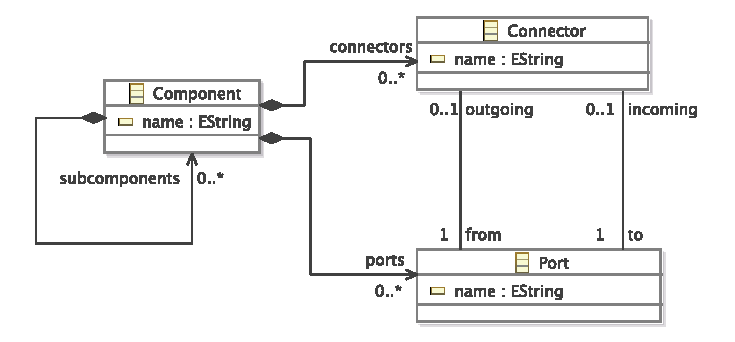
\includegraphics{images/FlockPOExampleOriginal.pdf}
    }
    \subbottom[Evolved metamodel.]
    {
        \label{fig:evolved_po_mm}
        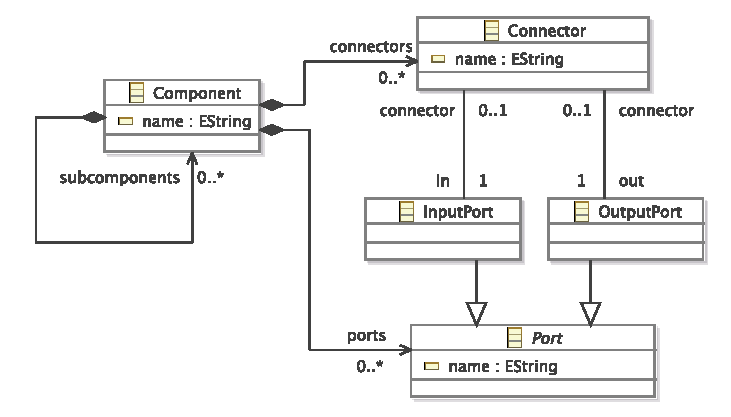
\includegraphics{images/FlockPOExampleEvolved.pdf}
    }
    \caption{Process-oriented metamodel evolution.}
    \label{fig:po_mms}
\end{figure}
%\end{landscape}

Some models that conform to the original metamodel do not conform to the evolved metamodel. Specifically, models might not conform to the evolved metamodel because:

\begin{enumerate}
	\item They contain instances of \texttt{Port}, which is an abstract class in the evolved metamodel.
	\item They contain instances of \texttt{Connector} that specify values for the features \texttt{to} and \texttt{from}, which are not defined for the \texttt{Connector} type in the evolved metamodel.
	\item They contain instances of \texttt{Connector} that do not specify a value for the \texttt{in} and \texttt{out} features, which are mandatory for the \texttt{Connector} type in the evolved metamodel.
\end{enumerate}

Model migration can be achieved with a general-purpose model-to-model transformation using a language such as ETL (Chapter~\ref{sec:ETL}). However, this typically involves writing a large amount of repetitive and redundant code \cite{rose12flock}. Flock reduces the amount of repetitive and redundant code needed to specify model migration by automatically copying from the original to the migrated model all of the model elements that conform to the evolved metamodel as described below.




%\begin{landscape}
\begin{sidewaysfigure}
	\centering
		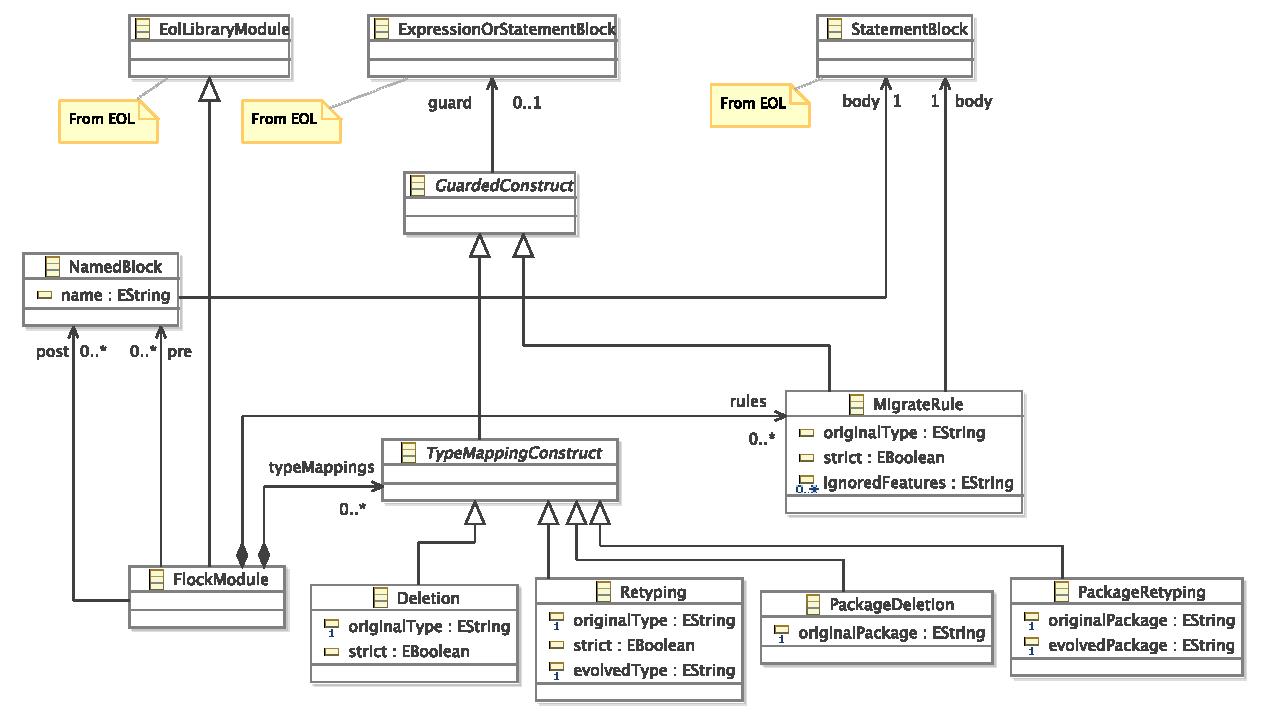
\includegraphics{images/FlockAbstractSyntax.pdf}
	\caption{The Abstract Syntax of Flock}
	\label{fig:flock_abstract_syntax}
\end{sidewaysfigure}
%\end{landscape}


\section{Abstract Syntax}

As illustrated by Figure~\ref{fig:flock_abstract_syntax}, Flock migration strategies are organised into individual modules (\texttt{Flo\-ckMo\-du\-le}). Flock modules inherit from EOL language constructs for specifying user-defined operations and for importing other (EOL and Flock) modules. Like the other rule-based of Epsilon, Flock modules may comprise any number of pre (post) blocks, which are executed before (after) all other constructs. Flock modules comprise any number of type mappings (\texttt{Ty\-peMa\-pp\-i\-ng}) and rules (\texttt{Ru\-le}). Type mappings operate on metamodel types (\texttt{Rety\-pi\-ng} and \texttt{De\-le\-ti\-on}) or on metamodel packages (\texttt{Pa\-ck\-a\-geRety\-pi\-ng} and \texttt{Pa\-ck\-a\-geDe\-le\-ti\-on}). Type mappings are applied to a type in the original metamodel (\texttt{or\-ig\-in\-alTy\-pe}) or to a package in the original metamodel (\texttt{or\-ig\-in\-alPa\-ck\-a\-ge}) . Additionally, \texttt{Rety\-pi\-ng}s apply to an evolved metamodel type (\texttt{ev\-ol\-vedTy\-pe}) or package (\texttt{ev\-ol\-vedPa\-ck\-a\-ge}). Each rule has an original metamodel type (\texttt{or\-ig\-in\-alTy\-pe}), a \texttt{bo\-dy} comprising a block of EOL statements, and zero or more \texttt{ig\-no\-r\-edFe\-at\-ur\-es}. Type mappings and rules can optionally specify a \texttt{gu\-ard}, which is either an EOL statement or a block of EOL statements. Type mappings that operate on metamodel types and rules can be marked as \texttt{str\-ict}.

\section{Concrete Syntax}

Listing \ref{lst:FlockConcreteSyntax} demonstrates the concrete syntax of the Flock language constructs. All of the constructs begin with keyword(s) (\texttt{retype}, \texttt{retype package} \texttt{delete}, \texttt{delete package} or \texttt{migrate}), followed by the original metamodel type or package. Additionally, type mappings that operate on metamodel types and rules can be annotated with the \texttt{strict} modifier. The \texttt{delete} construct can be annotated with a \texttt{cascade} modifier. All constructs can have guards, which are specified using the \texttt{when} keyword.

Migrate rules can specify a list of features that conservative copy will ignore (\texttt{ignoring}), and a \texttt{body} containing a sequence of at least one EOL statement. Note that a migrate rule must have a list of ignored features, or a body, or both.

\begin{lstlisting}[caption={Concrete syntax of Flock retypings, deletions and migrate rules}, label=lst:FlockConcreteSyntax, language=Flock, escapechar=!]
(@strict)?
retype !\textit{<originalType>}! to !\textit{<evolvedType>}!
(when (!\textbf{:}\textit{<eolExpression>}!)|(!\textbf{\{}\textit{<eolStatement>+}\textbf{\}}!))?

retype package !\textit{<originalPackage>}! to !\textit{<evolvedPackage>}!
(when (!\textbf{:}\textit{<eolExpression>}!)|(!\textbf{\{}\textit{<eolStatement>+}\textbf{\}}!))?

(@strict)?
(@cascade)?
delete !\textit{<originalType>}!
(when (!\textbf{:}\textit{<eolExpression>}!)|(!\textbf{\{}\textit{<eolStatement>+}\textbf{\}}!))?

delete package !\textit{<originalPackage>}!
(when (!\textbf{:}\textit{<eolExpression>}!)|(!\textbf{\{}\textit{<eolStatement>+}\textbf{\}}!))?

(@strict)?
migrate !\textit{<originalType>}!
(ignoring !\textit{<featureList>}!)?
(when (!\textbf{:}\textit{<eolExpression>}!)|(!\textbf{\{}\textit{<eolStatement>+}\textbf{\}}!))? {
	!\textit{<eolStatement>}!+
}
\end{lstlisting}

\emph{Pre} and \emph{post} blocks have a simple syntax that, as presented in Listing \ref{lst:FlockPrePostConcreteSyntax}, consists of the identifier (\emph{pre} or \emph{post}), an optional name and the set of statements to be executed enclosed in curly braces.

\begin{lstlisting}[caption=Concrete Syntax of Pre and Post blocks, label=lst:FlockPrePostConcreteSyntax, language=Flock]
(pre|post) <name> {
	statement+
}
\end{lstlisting}

\section{Execution Semantics}
The execution semantics of a Flock module are now described. Note that the Epsilon Model Connectivity (EMC) layer (Chapter~\ref{sec:Design.EMC}), which Flock uses to access and manipulate models supports a range of modelling technologies, and identifies types by name. Consequently, the term \emph{type} is used to mean ``the name of an element of a metamodel'' in the following discussion. For example, \texttt{Co\-mp\-on\-e\-nt}, \texttt{Co\-nn\-ec\-t\-or} and \texttt{In\-p\-utPo\-rt} are three of the types defined in Figure~\ref{fig:evolved_po_mm}.

Execution of a Flock module occurs in six phases:
\begin{enumerate}
  \item Any pre blocks are executed.
  \item Type mapping constructs (retypings and deletions) are processed to identify the way in which original and evolved metamodel types are to be related.
  \item Migrate rules are inspected to build sets of ignored properties.
  \item The information determined in steps 2 and 3 is used as input a copying algorithm, which creates an (equivalent) element in the migrated model for each element of the original model, and copies values from original to equivalent model elements.
  \item Migrate rules are executed on each pair of original and (equivalent) migrated model elements.
  \item Any post blocks are executed.
\end{enumerate}

In phases 2-5, language constructs are executed only when they are \emph{applicable}. The \emph{applicability} of the Flock language constructs (retyping, deletion or migrate rule) is determined from their type and guard. For a language construct $c$ to be applicable to an original model element $o$, $o$ must instantiate either the original type of $c$ or one of the subtypes of the original type of $c$; and $o$ must satisfy the guard of $c$. For language constructs that have been annotated as strict, type-checking is more restrictive: $o$ must instantiate the original type of $c$ (and not one its subtypes). In other words, the applicability of strict constructs is determined with EOL's \texttt{isTypeOf} operation and the applicability of non-strict constructs is determined with EOL's \texttt{isKindOf} operation (Table~\ref{tab:AnyOperations}). For language constructs that have been annotated with cascade, type-checking is less restrictive: $o$ must be contained in another model element (either directly or indirectly) to which the construct is applicable. Similarly, for language constructs that operate on packages (i.e. package retyping and package deletions), type-checking is less restrictive: $o$ must be contained in a package with the same name as the original package of $c$.

Phases 2-4 of execution implement a copying algorithm which has been termed conservative copy and is discussed thoroughly elsewhere \cite{rose12flock}. Essentially, conservative copy will do the following for each element of the original model, $o$:

\begin{enumerate}
	\item \textbf{Do nothing} when $o$ instantiates a type that cannot be instantiated in the evolved metamodel (e.g., because the type of $o$ is now abstract or no longer exists). Example: instances of \texttt{Port} in Figure~\ref{fig:po_mms} are not copied because \texttt{Port} has become abstract.
	\item \textbf{Fully copy} $o$ to produce $m$ in the migrated model when $o$ instantiate a type that has not been at all affected by metamodel evolution. Example: instances of \texttt{Component} in Figure~\ref{fig:po_mms} are fully copied because neither \texttt{Component} nor any of its features have been changed.
	\item \textbf{Partially copy} $o$ to produce $m$ in the migrated model when $o$ instantiates a type with one or more features that have been affected by metamodel evolution. Example: instances of \texttt{Connector} in Figure~\ref{fig:po_mms} are partially copied because the \texttt{from} and \texttt{to} features have been renamed. Note that in a partial copy only the features that have not been affected by metamodel evolution are copied (e.g., the \texttt{name}s of \texttt{Connector}s).
\end{enumerate}

In phase 5, migrate rules are applied. These rules specify the problem-specific migration logic and might, for example, create migrated model elements for original model elements that were skipped or partially copied by the copying algorithm described above. The Flock engine makes available two variables (\texttt{or\-ig\-in\-al} and \texttt{mi\-gr\-at\-ed}) for use in the body of any migration rule. These variables are used to refer to the particular elements of the original and migrated models to which the rule is currently being applied. In addition, Flock defines an \texttt{equivalent()} operation that can be called on any original model element and returns the equivalent migrated model element (or \texttt{null}). The \texttt{equivalent()} operation is used to access elements of the migrated model that cannot be accessed via the \texttt{migrated} variable due to metamodel evolution. Flock rules often contain statements of the form: \texttt{original.x.equivalent()} where \texttt{x} is a feature that has been removed from the evolved metamodel.

Finally, we should consider the order in which Flock schedules language constructs: a construct that appears earlier (higher) in the source file has priority. This is important because only one type mapping (retypings and deletions) is applied per original model element, and because this implies that migrate rules are applied from top-to-bottom. This ordering is consistent with the other languages of the Epsilon platform.


\section{Example}
Flock is now demonstrated using the example of model migration introduced in Section~\ref{sec:flock_background}. Recall that the metamodel evolution in Figure~\ref{fig:po_mms} involves splitting the \texttt{Po\-rt} type to form the \texttt{In\-p\-utPo\-rt} and \texttt{Ou\-tp\-utPo\-rt} types. Figure~\ref{fig:po_migration_strategy} provides a high-level design for migrating models from the original to the evolved metamodel in Figure~\ref{fig:po_mms}.

\begin{figure}[h]
    \begin{framed}
        \footnotesize
        \begin{itemize}
            \item For every instance, p, of \texttt{Port} in the original model: 
            \subitem $-$ If there exists in the original model a \texttt{Connector}, c, that specifies p as the value for its \texttt{from} feature:
            \subsubitem $-$ Create a new instance, i, of \texttt{InputPort} in the migrated model.
            \subsubitem $-$ Set c as the \texttt{connector} of i.
            \subsubitem $-$ Add c to the \texttt{ports} reference of the \texttt{Component} that contains c.
            
            \subitem $-$ If there exists in the original model a \texttt{Connector}, c, that specifies p as the value for its \texttt{to} feature:
            \subsubitem $-$ Create a new instance of \texttt{OutputPort} in the migrated model.
            \subsubitem $-$ Set c as the \texttt{connector} of i.
            \subsubitem $-$ Add c to the \texttt{ports} reference of the \texttt{Component} that contains c.
            
            \item And nothing else changes.
        \end{itemize}
    \end{framed}
    \caption{Model migration strategy in pseudo code for the metamodel evolution in Figure~\ref{fig:po_mms}.}
    \label{fig:po_migration_strategy}
\end{figure}

The Flock migration strategy that implements this design is shown\footnote{Note that \texttt{in} and \texttt{to} are reserved words in EOL, and hence backticks are used to refer to the metamodel features \texttt{in} and \texttt{to} on lines 7, 8 and 16 of Listing~\ref{lst:flock}.} in Listing~\ref{lst:flock}. Three type mappings constructs (on lines 1-4) are used to control the way in which instances of \texttt{Po\-rt} are migrated. For example, line 3 specifies that instances of \texttt{Po\-rt} that are referenced via the \texttt{fr\-om} feature of a \texttt{Co\-nn\-ec\-t\-or} are retyped, becoming \texttt{In\-pu\-tPo\-rt}s. Instances of \texttt{Co\-nn\-ec\-t\-or} are migrated using the rule on lines 6-9, which specifies the way in which the \texttt{fr\-om} and \texttt{to} features have evolved to form the \texttt{in} and \texttt{out} features.

\begin{lstlisting}[float=t,caption=Flock migration strategy for the process-oriented metamodel evolution in Figure~\ref{fig:po_mms}, label=lst:flock, language=Flock]
delete Port when: not (original.isInput() xor original.isOutput())

retype Port to InputPort  when: original.isInput()
retype Port to OutputPort when: original.isOutput()

migrate Connector {
migrated.`in` = original.from.equivalent();
migrated.out = original.`to`.equivalent();
}

operation Original!Port isInput() : Boolean {
return Original!Connector.all.exists(c|c.from == self);
}

operation Original!Port isOutput() : Boolean {
return Original!Connector.all.exists(c|c.`to` == self);
}
\end{lstlisting}


Note that metamodel elements that have not been affected by the metamodel evolution, such as \texttt{Co\-mp\-on\-e\-nt}s, are migrated automatically. Explicit copying code would be needed to achieve this with a general purpose model-to-model transformation language.

\section{Limitations and Scope}
Although Flock has been shown to much more concise than general purpose model-to-model transformation languages for specifying model migration, Flock does not provide some of the features commonly available in general-purpose model-to-model transformation language. This section discusses the limitations of Flock and its intended scope with respect to other tools for model migration.

\subsection{Limitations}
Firstly, Flock does not support rule inheritance, and re-use of migration logic is instead achieved by exploiting the inheritance hierarchy of the original metamodel. The form of re-use provided by Flock is less general than rule-inheritance, but has proved sufficient for existing use-cases.

Secondly, Flock does not provide language constructs for controlling the order in which rules are scheduled (other than the ordering of the rules in the program file). ATL, for example, includes constructs that allow users to specify that rules are scheduled explicitly (lazy rules) or in a memoised manner (unique rules). We anticipate that scheduling constructs might be necessary for larger migration strategies, but have not yet encountered situations in which they have been required.

Thirdly, Flock is tailored for applying migration to a single original and a single migrated model. Although further models can be accessed by a Flock migration strategy, they cannot be used as the source or target of the conservative copy algorithm. By contrast, some general-purpose model transformation languages can access and manipulate any number of models.

Finally, Flock has been tailored to the model migration problem. In other words, we believe that Flock is well-suited to specifying model transformations between two metamodels that are very similar. For metamodel evolution in which the original metamodel undergoes significant and large-scale revision, a general-purpose transformation might be more suitable than Flock for specifying model migration.

\subsection{Scope}
Flock is typically used as a manual specification approach in which model migration strategies are written by hand. As such, we believe that Flock provides a flexible and concise way to specify migration, and is a foundation for further tools that seek to automate the metamodel evolution and model migration processes. There are approaches to model migration that encompass both the metamodel evolution and model migration processes, seeking to automatically derive model migration strategies (e.g., Edapt \url{http://www.eclipse.org/edapt/}). These approaches provide more automation but at the cost of flexibility: for example, you might be restricted to using a tool-specific editor to perform model migration, or to using only EMF.


\section{Further Reading}
Further examples of applying Flock include migration of UML activity diagrams (at Transformation Tool Contest 2010 workshop\footnote{\url{http://planet-mde.org/ttc2010/}}), and migration of UML class diagrams, GMF models, and a domain-specific modelling language for NNTP newsgroups in Rose's doctoral thesis \cite{rose11thesis}.

A more thorough discussion of the design decisions and execution semantics of Flock can be found in a SoSyM journal article \cite{rose12flock}. Flock has been compared with other model migration tools and languages in a MoDELS paper \cite{rose10comparison}. 


\chapter{The Epsilon Pattern Language (EPL)}
\label{sec:EPL}

\section{Background and Motivation}
Several solutions have been proposed for the problem of pattern matching in models conforming to metamodels specified using standardised metamodelling languages. The majority of these solutions take the form of tailored graphical or textual languages, through which patterns can be specified at a certain level of abstraction, and accompanying interpreters/compilers which can then match these pattern specifications against concrete models. Examples of graphical pattern matching languages include AGG~\cite{AGG2004} and EMF Tiger~\cite{EMFTiger}, while examples of textual languages include GrGen.NET~\cite{GrGen}, VIATRA2~\cite{VIATRA2} and EMF-IncQuery~\cite{EMFIncQuery}. In \cite{QVTRPatterns}, QVTr has also been used to express and detect patterns in EMF models.

Pattern matching is often only one step in a chain of model management operations. As such, languages for pattern matching should ideally integrate seamlessly with languages that support other model management tasks such as model validation, comparison, transformation etc. In our review of previous work, we have identified that existing languages for pattern matching are typically bundled together with in-place and/or model-to-model transformation capabilities, and can only be integrated with languages that support other MDE tasks such as model validation and model-to-text transformation either through serialising detected patterns in a commonly supported format or through developing bespoke inter-tool adapters. Even in cases where interoperability with other model management languages is feasible, developing pattern specifications and other model management programs in different and inconsistent syntaxes can introduce code duplication and, consequently, hinder development and maintenance \cite{ICCECS09}. Another limitation of existing pattern matching languages is that they typically target a specific modelling technology (e.g. EMF) and/or model representation format, which renders specifying and detecting patterns that involve elements of heterogeneous models (e.g. an EMF model and an XML document) particularly challenging, if possible at all.

The above limitations have motivated us to design and implement a new pattern matching language, the Epsilon Pattern Language (EPL), which enables seamless runtime interoperability and code reuse with languages supporting a range of model management tasks, and also provides support for specifying patterns that involve elements of models conforming to different modelling technologies.

\newcommand {\omnigraffle}[1] {
\includegraphics[scale=0.55]{#1}
}

This chapter discusses the abstract and concrete syntax of EPL as well as its execution semantics. To aid understanding, the discussion of the syntax and the semantics of the language revolves around an exemplar pattern which is developed incrementally throughout the chapter. The exemplar pattern is matched against models extracted from Java source code using tooling provided by the MoDisco\footnote{http://www.eclipse.org/MoDisco/} project. MoDisco is an Eclipse project that provides a fine-grained Ecore-based metamodel of the Java language as well as tooling for extracting models that conform to this Java metamodel from Java source code. A simplified view of the relevant part of the MoDisco Java metamodel used in this running example is presented in Figure~\ref{fig:JavaMetamodel}.

The aim of the pattern developed in this chapter (which we will call \emph{PublicField}) is to identify quartets of $<$ClassDeclaration, FieldDeclaration, MethodDeclaration, MethodDeclaration$>$, each representing a field of a Java class for which appropriately named accessor/getter (getX/isX) and mutator/setter (setX) methods are defined by the class.

\begin{figure}[htbp]
\centering
\omnigraffle{images/Java.pdf}
\caption{Simplified view of the MoDisco Java metamodel}
\label{fig:JavaMetamodel}
\end{figure}

\section{Syntax}

The syntax of EPL is an extension of the syntax of the EOL language, which -- as discussed earlier -- is the core language of Epsilon. As such, any references to \emph{expression} and \emph{statement block} in this chapter, refer to EOL expressions and blocks of EOL statements respectively. It is also worth noting that EOL expressions and statements can produce side-effects on models, and therefore, it is the responsibility of the developer to decide which expressions used in the context of EPL patterns should be side-effect free and which not.

As illustrated in Figure \ref{fig:EPLAbstractSyntax}, EPL patterns are organised in \emph{modules}. Each module contains a number of named \emph{patterns} and optionally, \emph{pre} and \emph{post} statement blocks that are executed before and after the pattern matching process, and helper EOL operations. EPL modules can import other EPL and EOL modules to facilitate reuse and modularity.

\begin{figure}[htbp]
\centering
\omnigraffle{images/EPL.pdf}
\caption{Abstract Syntax of EPL}
\label{fig:EPLAbstractSyntax}
\end{figure}

In its simplest form a \emph{pattern} consists of a number of named and typed \emph{roles} and a \emph{match} condition. For example, in lines \ref{components-start}-\ref{components-end}, the \emph{PublicField} pattern of Listing \ref{lst:Example}, defines four roles (\emph{class}, \emph{field}, \emph{setter} and \emph{getter}). The \emph{match} condition of the pattern specifies that for a quartet to be a valid match, the field, setter and getter must all belong to the class (lines \ref{belongs-start}-\ref{belongs-end}), and that the setter and getter methods must be appropriately named\footnote{To maintain the running example simple and concise, the pattern does not check aspects such as matching/compatible parameter/return types in the field, setter and getter but the reader should easily be able to envision how this would be supported through additional clauses in the match condition.}.
\clearpage
\begin{lstlisting}[flexiblecolumns=true, nolol=false, caption=First version of the PublicField pattern, label=lst:Example, breaklines=true, language=EPL, escapeinside={@*}{*@}]
pattern PublicField
	class : ClassDeclaration, field : FieldDeclaration, @*\label{components-start}*@
	setter : MethodDeclaration, getter : MethodDeclaration { @*\label{components-end}*@
	
	match : class.bodyDeclarations.includes(field) and @*\label{belongs-start}*@ @*\label{match-start}*@
		class.bodyDeclarations.includes(setter) and
		class.bodyDeclarations.includes(getter) and @*\label{belongs-end}*@
		setter.name = "set" + field.getName() and
		(getter.name = "get" + field.getName() or
		getter.name = "is" + field.getName()) @*\label{match-end}*@
}

@cached
operation FieldDeclaration getName() {
	return self.fragments.at(0).name.firstToUpperCase();
}
\end{lstlisting}

The implementation of the PublicField pattern provided in Listing \ref{lst:Example} is fully functional but not particularly efficient as the \emph{match} condition needs to be evaluated $\#ClassDefinition * \#FieldDeclaration * \#MethodDeclaration^{2}$ times. To enable pattern developers to reduce the search space, each \emph{role} in an EPL pattern can specify a \emph{domain} which is an EOL expression that returns a collection of model elements from which the role will draw values.

There are two types of domains in EPL: static domains which are computed once for all applications of the pattern, and which \textbf{are not} dependent on the bindings of other roles of the pattern (denoted using the \emph{in} keyword in terms of the concrete syntax), and dynamic domains which are recomputed every time the candidate values of the role are iterated, and which \textbf{are} dependent on the bindings of other roles (denoted using the \emph{from} keyword). Beyond a domain, each role can also specify a \emph{guard} expression that further prunes unnecessary evaluations of the match condition. Using dynamic domains and guards, the \emph{PublicField} pattern can be expressed in a more efficient way, as illustrated in Listing \ref{lst:Example2}. To further illustrate the difference between dynamic and static domains, changing \emph{from} to \emph{in} in line \ref{dynamicdomain} would trigger a runtime exception as the domain would become static and therefore not able to access bindings of other roles (i.e. \emph{class}).
\clearpage
\begin{lstlisting}[flexiblecolumns=true, nolol=false, caption=Second version of the PublicField pattern using domains and guards, label=lst:Example2, breaklines=true, language=EPL, escapeinside={@*}{*@}]
pattern PublicField
	class : ClassDeclaration,
	field : FieldDeclaration
		from: class.bodyDeclarations, @*\label{dynamicdomain}*@
	setter : MethodDeclaration
		from: class.bodyDeclarations
		guard: setter.name = "set" + field.getName(),
	getter : MethodDeclaration
		from: class.bodyDeclarations 
		guard : (getter.name = "get" + field.getName() or
		         getter.name = "is" + field.getName()) { }
\end{lstlisting}

The implementation of Listing \ref{lst:Example2} is significantly more efficient than the previous implementation but can still be improved by further reducing the number of name comparisons of candidate \emph{setter} and \emph{getter} methods. To achieve this we can employ memoisation: we create a hash map of method names and methods once before pattern matching (line \ref{example3-pre}), and use it to identify candidate setters and getters (lines \ref{example3-setter-from} and \ref{example3-getter-from}-\ref{example3-getter-from2}).

\begin{lstlisting}[flexiblecolumns=true, nolol=false, caption=Third version of the PublicField pattern, label=lst:Example3, breaklines=true, language=EPL, escapeinside={@*}{*@}]
pre {
	var methodMap = MethodDeclaration.all.mapBy(m|m.name); @*\label{example3-pre}*@
}
pattern PublicField
	class : ClassDeclaration,
	field : FieldDeclaration
		from: class.bodyDeclarations,
	setter : MethodDeclaration @*\label{example3-setter}*@
		from: getMethods("set" + field.getName()) @*\label{example3-setter-from}*@
		guard: setter.abstractTypeDeclaration = class,
	getter : MethodDeclaration
		from: getMethods("get" + field.getName()) @*\label{example3-getter-from}*@
				.includingAll(getMethods("is" + field.getName())),  @*\label{example3-getter-from2}*@
		guard: getter.abstractTypeDeclaration = class {
}

operation getMethods(name : String) : Sequence(MethodDeclaration) {
	var methods = methodMap.get(name);
	if (methods.isDefined()) return methods;
	else return new Sequence;
}
\end{lstlisting}

The sections below discuss the remainder of the syntax of EPL.

\subsection{Negative Roles}
Pattern roles can be negated using the \emph{no} keyword. For instance, by adding the \emph{no} keyword before the setter role in line \ref{example3-setter} of Listing \ref{lst:Example3}, the pattern will match fields that have getters but no setters (i.e. read-only fields).

\subsection{Optional and Active Roles}
Pattern roles can be designated as optional using the \emph{optional} EOL expression. For example, adding \texttt{optional: true} to the setter role would also match all fields that only have a getter. By adding \texttt{optional: true} to the setter role and \texttt{optional: setter.isDefined()} to the getter role, the pattern would match fields that have at least a setter or a getter. Roles can be completely deactivated depending on the bindings of other roles through the \emph{active} construct. For example, if the pattern developer prefers to specify separate roles for \emph{getX} and \emph{isX} getters, with a preference over getX getters, the pattern can be formulated as illustrated in Listing \ref{lst:Example4} so that if a \emph{getX} getter is found, no attempt is even made to match an \emph{isX} getter.

\begin{lstlisting}[flexiblecolumns=true, nolol=false, caption=PublicField Pattern Version 4, label=lst:Example4, breaklines=true, language=EPL, escapeinside={@*}{*@}]
pattern PublicField
	class : ClassDeclaration,
	field : FieldDeclaration ...,
	setter : MethodDeclaration ...,
	getGetter : MethodDeclaration ...,
	isGetter: MethodDeclaration
		...
		active: getGetter.isUndefined() {
}
\end{lstlisting}

\subsection{Role Cardinality}
The cardinality of a role (lower and upper bound) can be defined in square brackets following the type of the role. Roles that have a cardinality with an upper bound $>$ 1 are bound to the subset of elements from the domain of the role which also satisfy the guard, if the size of that subset is within the bounds of the role's cardinality. Listing \ref{lst:Cardinality} demonstrates the \emph{ClassAndPrivateFields} pattern that detects instances of classes and all their private fields. If the cardinality of the field role in line \ref{field-cardinality} was [1..3] instead of [*], the pattern would only detect classes that own 1 to 3 private fields.

\clearpage
\begin{lstlisting}[flexiblecolumns=true, nolol=false, caption=Demonstration of Role Cardinality, label=lst:Cardinality, breaklines=true, language=EPL, escapeinside={@*}{*@}]
pattern ClassAndPrivateFields
	class : ClassDeclaration,
	field : FieldDeclaration[*]  @*\label{field-cardinality}*@
		from: class.bodyDeclarations
		guard: field.getVisibility() = VisibilityKind#private {
	
	onmatch { @*\label{onmatch-start}*@
	 	var message : String;
	 	message = class.name + " matches";
	 	message.println();
	} @*\label{onmatch-end}*@
	
	do { @*\label{do}*@
		// More actions here
	}
	
	nomatch : (class.name + " does not match").println() @*\label{nomatch}*@
}
operation FieldDeclaration getVisibility() {
	if (self.modifier.isDefined()) {
		return self.modifier.visibility; }
	else { return null; }
}
\end{lstlisting}

\section{Execution Semantics}
When an EPL module is executed, all of its \emph{pre} statement blocks are first executed in order to define and initialise any global variables needed (e.g. the \emph{methodMap} variable in Listing \ref{lst:Example3}) or to print diagnostic messages to the user. Subsequently, patterns are executed in the order in which they appear. For each pattern, all combinations that conform to the type and constraints of the roles of the pattern are iterated, and the validity of each combination is evaluated in the \emph{match} statement block of the pattern. In the absence of a \emph{match} block, every combination that satisfies the constraints of the roles of the pattern is accepted as a valid instance of the pattern.

Immediately after every successful match, the optional \emph{onmatch} statement block of the pattern is invoked (see lines \ref{onmatch-start}-\ref{onmatch-end} of Listing \ref{lst:Cardinality}) and after every unsuccessful matching attempt, for combinations which however satisfy the constraints specified by the roles of the pattern, the optional \emph{nomatch} statement block of the pattern (line \ref{nomatch}) is executed . When matching of all patterns is complete, the \emph{do} part (line \ref{do}) of each successful match is executed. In the \emph{do} part, developers can modify the involved models (e.g to perform in-place transformation), without the risk of concurrent list modification errors (which can occur if elements are created/deleted during pattern matching). After pattern matching has been completed, the \emph{post} statement blocks of the module are executed in order to perform any necessary finalisation actions.

An EPL module can be executed in a one-off or iterative mode. In the one-off mode, patterns are only evaluated once, while in the iterative mode, the process is repeated until no more matches have been found or until the maximum number of iterations (specified by the developer) has been reached. The iterative mode is particularly suitable for patterns that perform reduction of the models they are evaluated against.

\section{Pattern Matching Output}

The output of the execution of an EPL module on a set of models is a collection of matches encapsulated in a \emph{PatternMatchModel}, as illustrated in Figure \ref{fig:PatternMatchModel}. As \emph{PatternMatchModel} implements the \emph{IModel} interface discussed in Chapter \ref{sec:Design.EMC}, its instances can be accessed from other programs expressed in languages of the Epsilon family.

\begin{figure}[htbp]
\begin{center}
\omnigraffle{images/PatternMatchModel.pdf}
\caption{Pattern Matching Output}
\label{fig:PatternMatchModel}
\end{center}
\end{figure}

A \emph{PatternMatchModel} introduces one model element type for each pattern and one type for each field of each pattern (the name of these types are derived by concatenating the name of the pattern with a camel-case version of the name of the field). Instances of the prior are the matches of the pattern while instances of the latter are elements that have been matched in this particular role. For example, after executing the EPL module of Listing \ref{lst:Example3}, the produced \emph{PatternMatchModel} contains 5 types: \emph{PublicField}, instances of which are all the identified matches of the \emph{PublicField} pattern, \emph{PublicFieldClass}, instances of which are all the classes in the input model which have been matched to the \emph{class} role in instances of the \emph{PublicField} pattern, and similarly \emph{PublicFieldField}, \emph{PublicFieldSetter} and \emph{PublicFieldGetter}. 

\section{Interoperability with Other Model Management Tasks}

As a \emph{PatternMatchModel} is an instance of \emph{IModel}, after its computation it can be manipulated by other Epsilon programs. For example, Listing \ref{lst:ANT} demonstrates running the EPL module of Listing \ref{lst:Example3} and passing its output to the EVL constraints module of Listing \ref{lst:EVL} and, if validation is successful, to an ETL transformation where it is used to guide the generation of a UML model.

In lines \ref{ant-loadmodel-start}-\ref{ant-loadmodel-end} of Listing \ref{lst:ANT} (see Chapter \ref{chp:Workflow} for a detailed discussion on the Epsilon ANT tasks), the Java model is loaded and is assigned the name \emph{Java}. Then, in line \ref{ant-epl-start}, the \emph{Java} model is passed on to \emph{publicfield.epl} for pattern matching. The result of pattern matching, which is an instance of the \emph{PatternMatchModel} class (and therefore also an instance of \emph{IModel}) is exported to the global context under the name \emph{Patterns}. Then, in lines \ref{ant-evl-start}, both the \emph{Patterns} and the \emph{Java} are passed on to the EVL model validation task which performs validation of the identified pattern matches.

\begin{lstlisting}[flexiblecolumns=true, nolol=false, caption=ANT workflow calculating and passing a pattern match model to an EVL validation module, label=lst:ANT, breaklines=true, language=XML, escapeinside={@*}{*@}]
<project default="main">
	<target name="main">
	
		<epsilon.emf.loadModel name="Java" @*\label{ant-loadmodel-start}*@
			modelfile="org.eclipse.epsilon.eol.engine_java.xmi" 
			metamodeluri="...MoDisco/Java/0.2.incubation/java"
			read="true" store="false"/> @*\label{ant-loadmodel-end}*@
		
		<epsilon.epl src="publicfield.epl" exportAs="Patterns"> @*\label{ant-epl-start}*@
			<model ref="Java"/>
		</epsilon.epl> @*\label{ant-epl-end}*@
		
		<epsilon.evl src="constraints.evl"> @*\label{ant-evl-start}*@
			<model ref="Patterns"/>
			<model ref="Java"/>
		</epsilon.evl> @*\label{ant-evl-end}*@

		<epsilon.etl src="java2uml.etl"> @*\label{ant-etl-start}*@
			<model ref="Patterns"/>
			<model ref="Java"/>
		</epsilon.etl> @*\label{ant-etl-end}*@
	</target>
</project>
\end{lstlisting}

Line \ref{ant-evl-context} of Listing \ref{lst:EVL} defines a set of constraints that will be applied to instances of the \emph{PublicField} type from the \emph{Patterns} model. As discussed above, these are all matched instances of the \emph{PublicField} pattern. Line \ref{ant-evl-check}, specifies the condition that needs to be satisfied by instances of the pattern. Notice the \emph{self.getter} and \emph{self.field} expressions which return the \emph{MethodDeclaration} and \emph{FieldDeclaration} bound to the instance of the pattern. Then, line \ref{ant-evl-message} defines the message that should be produced for instances of \emph{PublicField} that do not satisfy this constraint.
 
\begin{lstlisting}[flexiblecolumns=true, nolol=false, caption=Fragment of the constraints.evl EVL constraints module, label=lst:EVL, breaklines=true, language=EVL, escapeinside={@*}{*@}]
context Patterns!PublicField { @*\label{ant-evl-context}*@
	guard: self.field.type.isDefined()
	constraint GetterAndFieldSameType { 
		check : self.getter.returnType.type = self.field.type.type @*\label{ant-evl-check}*@
		message : "The getter of " + self.class.name + "." @*\label{ant-evl-message}*@
			+ self.field.fragments.at(0).name +
			" does not have the same type as the field itself"
	}
}
\end{lstlisting}

If validation is successful, both the \emph{Java} and the \emph{Patterns} model are passed on to an ETL transformation that transforms the \emph{Java} model to a UML model, a fragment of which is presented in Listing \ref{lst:ETL}. The transformation encodes $<field, setter, getter>$ triplets in the \emph{Java} model as public properties in the UML model. As such, in line \ref{etl-instanceof} of the transformation, the \emph{Patterns} model is used to check whether field \emph{s} has been matched under the \emph{PublicField} pattern, and if so, the next line ignores the field's declared visibility and sets the visibility of the respective UML property to \emph{public}.

\begin{lstlisting}[flexiblecolumns=true, nolol=false, caption=Fragment of the java2uml.etl Java to UML ETL transformation, label=lst:ETL, breaklines=true, language=ETL, escapeinside={@*}{*@}]
rule FieldDeclaration2Property
	transform s: Java!FieldDeclaration
	to t: Uml!Property {
	
	t.name = s.getName();
	if (s.instanceOf(Patterns!PublicFieldField)) { @*\label{etl-instanceof}*@
		t.visibility = Uml!VisibilityKind#public;
	}
	else {
		t.visibility = s.toUmlVisibility();
	}
	...
}
\end{lstlisting}

As Epsilon provides ANT tasks for all its languages, the same technique can be used to pass the result of pattern matching on to model-to-text transformations, as well as model comparison and model merging programs.


\chapter{Implementing a New Task-Specific Language}
\label{sec:Design.ImplementingANewLanguage}

Although Epsilon already provides languages for a wide range of model management tasks, additional tasks that could benefit from the convenience syntax and dedicated semantics of a task-specific language are likely to be identified in the future. Thus, this section distils the experiences obtained through the construction of existing task-specific languages to provide guidance on how to identify a task for which a dedicated language can be beneficial and develop the respective task-specific language for it atop the infrastructure provided by Epsilon.

\section{Identifying the need for a new language}

The first step of the process of constructing a new task-specific language is to identify a specific task for which a dedicated language is more appropriate than the general-purpose EOL. Typically, recurring syntactic and semantic patterns that emerge when attempting to implement the task using EOL indicate that a new task-specific language may be useful.

For example, before the introduction of the Epsilon Comparison Language, pure EOL was being used to perform model comparison. A simple comparison specification that establishes name-based matches between classes/attributes and tables/columns between two OO and DB models respectively using EOL is demonstrated in Listing \ref{lst:ComparisonEOL}.

Two patterns can be readily detected by inspecting the EOL code in Listing \ref{lst:ComparisonEOL}. First, explicit variables (\emph{matchingCT}, \emph{matchingAT}) are defined to capture the matching elements (class-table and attribute-column)identified during the comparison process. Also, to check all elements of one type (classes against tables and attributes against columns) repeated for statements are used in lines \ref{line:For11}--\ref{line:For12} and \ref{line:For21}--\ref{line:For22}. By contrast, Listing \ref{lst:ComparisonECL} which is specified using the task-specific ECL language does not include such low-level information. Instead it defines only the types of elements that need to be compared and the criteria on which comparison must performed and leaves the mundane tasks of scheduling and maintaining the match trace to the execution engine.

\begin{lstlisting}[caption=Comparing an OO model with a DB model using EOL, label=lst:ComparisonEOL, language=EOL]
var matchingCT : Sequence; /*@\label{line:MatchTrace1}@*/
var matchingAC : Sequence; /*@\label{line:MatchTrace2}@*/
for (c in OO!Class.allInstances) { /*@\label{line:For11}@*/
	for (t in DB!Table.allInstances) { /*@\label{line:For12}@*/
		if (t.name = c.name) {
			matchingCT.add(Sequence{c,t});
			for (att in c.attributes) { /*@\label{line:For21}@*/
				for (col in t.columns) { /*@\label{line:For22}@*/
					if (att.name = c.name) {
						matchingAC.add(Sequence{att, col});
					}
				}
			}
		}
	}
}
\end{lstlisting}

\begin{lstlisting}[caption=Comparing an OO model with a DB model using ECL, label=lst:ComparisonECL, language=ECL]
rule ClassTable
	match c : OO!Class
	with t : DB!Table {
	
	compare : c.name = t.name
}

rule AttributeColumn
	match a : OO!Attribute 
	with c : DB!Column {
	
	compare : a.name = c.name and
		a.class.matches(c.table)
}
\end{lstlisting}

\section{Eliciting higher-level constructs from recurring patterns}

Once recurring patterns, such as those discussed above, have been identified, the next step of the process is to derive higher level constructs from them. For instance, in the previous example, the nested for loops and the explicit trace variable declaration and population have been replaced by task-specific match rules.

Introducing higher-level involves defining its abstract and concrete syntax as well as its connection points with the underlying infrastructure. For example, in the case of ECL, the types of match rules are EOL model element types, the \emph{guard} and \emph{check} parts of a rule are EOL expressions or statements blocks and the \emph{pre} and \emph{post} blocks as well as the \emph{do} part of each rule are blocks of EOL statements.

\section{Implement Execution Semantics and Scheduling}

Once higher-level constructs (e.g. task-specific rules) have been identified and specified, their execution semantics and scheduling must be implemented similarly to what has been done for existing languages. Development of existing languages has demonstrated that task-specific constructs often need to provide more than one modes of execution (e.g. the \emph{lazy} and \emph{greedy} modes of ETL transformation rules discussed in Section \ref{sec:ETL.ExecutionSemantics}). 

A lightweight way to easily provide new execution modes and semantics for rules and user-defined operations without modifying the syntax of the language and introducing new keywords that may conflict with existing code, is through the annotations mechanism provided by EOL (see Section \ref{sec:Design.EOL.Annotations}). This approach has been adopted for the definition a small unit-testing language (EUnit), which is discussed in detail in \cite{EUnit}.

\section{Overriding Semantics}

In certain cases, it is useful to modify the semantics of certain constructs in EOL to meet the purposes of the task-specific language. An example of such a modification occurs in EVL where -- as discussed in Section \ref{sec:Design.EVL.ExecutionSemantics} -- the scope of the variables defined in \emph{guard} expression/block is extended so that variables can be reused in the context of non-nested blocks such as the \emph{title}, and \emph{check} parts of the invariant. Another example of overriding the semantics of EOL is the implementation of the special assignment operator ($::=$) by ETL which was discussed in \ref{sec:Design.ETL.SpecialAssignmentOperator}.




